% BAO CAO BTL - CSE703093 An toan phan mem
% DuongUniversity Management System - Module tinh tien giang vien
\documentclass[twoside,final]{phenikaa-report}

\usepackage{tgtermes}  % Times New Roman-like font with Vietnamese support

% Better tables
\usepackage{array,longtable,multicol,multirow,tabularx}
\usepackage{xcolor}
\usepackage{listings}

% Graphics
\usepackage{caption,float}
\usepackage[export]{adjustbox}

% References
\usepackage[nameinlink]{cleveref}

\graphicspath{{diagrams/}{graphics/}}

% Cho phep LaTeX gian dong nhe hon truoc khi bao Overfull \hbox, tranh tran le
% do cac ten ham \texttt{} dai (vd create_class_section_VULN()) khong the ngat dong.
\emergencystretch=3em
\tolerance=1000

% ===== Lightweight C listing style (no shell-escape / minted dependency) =====
\definecolor{codebg}{RGB}{245,244,240}
\definecolor{codekw}{RGB}{130,50,160}
\definecolor{codecm}{RGB}{0,120,0}
\definecolor{codestr}{RGB}{160,60,60}
\lstdefinestyle{cstyle}{
  language=C,
  backgroundcolor=\color{codebg},
  basicstyle=\ttfamily\footnotesize,
  keywordstyle=\color{codekw}\bfseries,
  commentstyle=\color{codecm}\itshape,
  stringstyle=\color{codestr},
  numbers=left,
  numberstyle=\tiny\color{gray},
  numbersep=6pt,
  frame=single,
  breaklines=true,
  showstringspaces=false,
  tabsize=2,
  captionpos=b
}
\lstset{style=cstyle}

% ===== Cover page configuration =====
\uniname{BỘ GIÁO DỤC VÀ ĐÀO TẠO}
\deptname{ĐẠI HỌC PHENIKAA}
\coursename{Học phần: CSE703093 -- An toàn phần mềm}
\reporttype{BÁO CÁO BÀI TẬP LỚN}
\title{End-to-end testing cho hệ thống tính tiền giảng dạy}
\advisor{ThS. Vũ Quang Dũng}
\stuname{%
  Nguyễn Minh Dương -- MSSV: 23010441 \\
  Đỗ Hữu Ngọc -- MSSV: 23010822
}
\reportplace{Hà Nội}
\reporttime{tháng 9 năm 2026}

\AtBeginDocument{\renewcommand{\contentsname}{Mục lục}}
\AtBeginDocument{\renewcommand{\listfigurename}{Danh mục hình ảnh}}
\AtBeginDocument{\renewcommand{\listtablename}{Danh mục bảng}}
\AtBeginDocument{\renewcommand{\tablename}{Bảng}}
\AtBeginDocument{\renewcommand{\figurename}{Hình}}
\AtBeginDocument{\renewcommand{\refname}{Tài liệu tham khảo}}
\AtBeginDocument{\renewcommand{\lstlistlistingname}{Danh mục mã nguồn}}
\AtBeginDocument{%
  \crefname{section}{mục}{mục}\Crefname{section}{Mục}{Mục}%
  \crefname{subsection}{mục}{mục}\Crefname{subsection}{Mục}{Mục}%
  \crefname{table}{bảng}{bảng}\Crefname{table}{Bảng}{Bảng}%
  \crefname{figure}{hình}{hình}\Crefname{figure}{Hình}{Hình}%
  \crefname{equation}{công thức}{công thức}\Crefname{equation}{Công thức}{Công thức}%
}

\begin{document}
\coverpage%

\tableofcontents
\listoffigures
\listoftables
\lstlistoflistings

\clearpage
\section{Giới thiệu và Mục tiêu}
\label{sec:gioithieu}

\subsection{Bối cảnh}

Các hệ thống quản lý đào tạo đại học quy mô lớn -- như \textbf{DuongUniversity Management System} -- xử lý đồng thời dữ liệu nhân sự (giảng viên), dữ liệu học vụ (lớp học phần) và dữ liệu tài chính (thù lao giảng dạy). Khi ba loại dữ liệu này liên thông với nhau qua các mô-đun C tốc độ cao (thường dùng ở tầng tính toán/tích hợp phía sau một backend .NET/PostgreSQL), một lỗi thao tác bộ nhớ ở mô-đun đầu (ví dụ giải phóng bộ nhớ giảng viên không đúng cách) có thể lan truyền thành lỗi tài chính nghiêm trọng ở mô-đun cuối (tính sai hoặc tính nhầm thù lao). Đây chính là rủi ro an toàn đặc trưng của hệ thống quản lý tài chính giáo dục: hậu quả của một lỗi an toàn bộ nhớ không dừng lại ở việc chương trình crash, mà có thể trở thành một quyết định tài chính sai (trả nhầm lương, từ chối duyệt lương cho giảng viên đã dạy thật).

Đề tài chọn đúng \textbf{mô-đun tính thù lao giảng viên} (\texttt{tinh\_tien\_day.c}, liên kết với \texttt{giang\_vien.c} và \texttt{lop\_hoc\_phan.c}) làm đối tượng phân tích vì đây là nơi hội tụ đầy đủ các đặc điểm cần thiết để một bài tập lớn an toàn phần mềm có ý nghĩa thực chất: (1) \textbf{xử lý input người dùng trực tiếp} (họ tên, bằng cấp, mã lớp qua \texttt{stdin}); (2) \textbf{thao tác con trỏ xuyên mô-đun} (\texttt{LopHocPhan.gv\_ptr} trỏ chéo sang \texttt{GiangVien}); và (3) \textbf{phép toán tài chính có thể tràn số} (nhân dồn số tiết, hệ số, đơn giá). Ba đặc điểm này tạo thành một \emph{attack surface} rõ ràng, đủ nhỏ để phân tích triệt để bằng 4 kỹ thuật kiểm chứng khác nhau, nhưng đủ thật để không chỉ là bài tập minh họa.

\subsection{Mục tiêu cụ thể}

Bài tập lớn đặt ra 4 mục tiêu cụ thể, mỗi mục tiêu ứng với một chương kỹ thuật, áp dụng trọn vẹn khung 4 chương công cụ của học phần~\cite{softsectoolkit2026} lên đúng một hệ thống E2E thay vì các bài tập minh hoạ độc lập:

\begin{enumerate}
  \item \textbf{Phát hiện lỗ hổng bộ nhớ và dữ liệu bằng phân tích tĩnh}: quét trực tiếp mã nguồn C, phát hiện tối thiểu 6 lớp lỗ hổng -- \textbf{CWE-120} (Buffer Copy without Checking Size), \textbf{CWE-416} (Use-After-Free), \textbf{CWE-476} (NULL Pointer Dereference), \textbf{CWE-190} (Integer Overflow), \textbf{CWE-1288} (Improper Validation of Specified Quantity/Enum), và \textbf{CWE-197} (Numeric Truncation Error) -- không cần biên dịch hay chạy chương trình.
  \item \textbf{Kiểm chứng luồng nghiệp vụ bằng mô hình hóa hình thức}: dựng mô hình Kripke $M=(S,S_0,R,L)$ cho luồng E2E 3 mô-đun và kiểm chứng bằng Bounded Model Checking (BMC, $k=5$) trên 5 thuộc tính LTL/CTL.
  \item \textbf{Chứng minh (hoặc bác bỏ) an toàn số học trên toàn miền giá trị bằng SMT}: dùng Z3 solver chứng minh phép tính thù lao có/không thể tràn số 32-bit, và chứng minh hình thức (không chỉ test mẫu) rằng bản vá loại trừ hoàn toàn lỗi.
  \item \textbf{Xác nhận lỗ hổng biểu hiện thật trên binary đã biên dịch bằng fuzzing động}: black-box (input ngẫu nhiên, đo crash rate thật trên \texttt{salary\_calc.exe}) và white-box (Z3-guided, giải trực tiếp điều kiện gây lỗi).
\end{enumerate}

\subsection{Phạm vi}

\textbf{Sẽ thực hiện:} phân tích, mô hình hóa và kiểm chứng 3 file module C -- \texttt{giang\_vien.c} (Module 1 -- Quản lý Giảng viên), \texttt{lop\_hoc\_phan.c} (Module 2 -- Quản lý Lớp học phần), \texttt{tinh\_tien\_day.c} (Module 3 -- Tính tiền dạy \& Thanh toán) -- cùng 2 driver \texttt{main.c} (bản có lỗ hổng cố ý, VULN) và \texttt{main\_fixed.c} (bản đã khắc phục, SAFE, dùng chung 3 module với bản VULN). Toàn bộ 4 chương công cụ (\texttt{ch1\_models}, \texttt{ch2\_memsafe}, \texttt{ch3\_staticsat}, \texttt{ch4\_dynafuzz}) đều áp dụng trên đúng 3 module này, đảm bảo tính nhất quán E2E thay vì 4 ví dụ minh họa rời rạc không liên quan tới nhau.

\textbf{Sẽ không thực hiện:} triển khai/kiểm chứng backend .NET 9 Web API, frontend React, hay kết nối cơ sở dữ liệu PostgreSQL thực của hệ thống DuongUniversity Management System -- các thành phần này chỉ được mô tả ở mức kiến trúc tổng quan (\Cref{sec:motahethong}) để xác định đúng vị trí của 3 module C trong hệ thống thật, không nằm trong phạm vi kiểm chứng của đề tài.

\section{Đặc tả Yêu cầu (Specification)}
\label{sec:dacta}

Trước khi phân tích lỗ hổng, đề tài đặc tả tường minh \emph{vùng input hợp lệ} và các quy tắc an toàn mà 3 module bắt buộc phải tuân thủ. Đây là cơ sở để mọi kỹ thuật kiểm chứng ở \Cref{sec:phuongphap} trả lời cùng một câu hỏi cốt lõi: \emph{``Mô-đun có chịu được khi input vượt ra ngoài vùng an toàn (đặc tả) hay không?''} -- thay vì chỉ hỏi ``output có đúng không'' trên một vài trường hợp thử.

\subsection{Bảng yêu cầu chức năng và phi chức năng}

\begin{table}[H]
  \centering
  \caption{Yêu cầu chức năng (functional) và an toàn (safety/memory) của hệ thống}
  \label{tab:req}
  \footnotesize
  \begin{tabularx}{\linewidth}{@{}l l l X@{}}
    \toprule
    \textbf{Mã YC} & \textbf{Loại} & \textbf{Ưu tiên} & \textbf{Nội dung đặc tả} \\
    \midrule
    REQ-1 & Safety & HIGH & Không được tính tiền khi chưa phân công giảng viên cho lớp học phần \\
    REQ-2 & Safety & HIGH & Không được xuất báo cáo khi chưa tính tiền \\
    REQ-3 & Memory & HIGH & \texttt{hoTen[80]}, \texttt{bangCap[20]}, \texttt{maLop[20]} không tràn bộ đệm khi input vượt kích thước (CWE-120) \\
    REQ-4 & Memory & HIGH & Con trỏ \texttt{gv\_ptr} (Module 2 $\to$ 1) không được truy cập sau khi vùng nhớ đã \texttt{free()} (CWE-416) \\
    REQ-5 & Memory & HIGH & \texttt{gv\_ptr} phải được kiểm tra \texttt{NULL} trước khi dùng để tính tiền (CWE-476) \\
    REQ-6 & Memory & HIGH & Phép nhân dồn số tiết $\times$ hệ số $\times$ đơn giá không tràn số nguyên 32-bit (CWE-190) \\
    REQ-7 & Functional & MEDIUM & Công thức tính tiền 2 bước phải cho kết quả đúng với mọi tổ hợp đầu vào hợp lệ \\
    REQ-8 & Integrity & HIGH & \texttt{soLuongSinhVien} (\texttt{int}) không sai lệch khi đóng gói vào audit log (\texttt{char}) (CWE-197) \\
    REQ-9 & Functional & MEDIUM & \texttt{bangCap} phải thuộc danh mục hợp lệ, không âm thầm rơi vào hệ số mặc định (CWE-1288) \\
    \bottomrule
  \end{tabularx}
\end{table}

\Cref{tab:req} là yêu cầu \emph{chức năng} (hệ thống làm \emph{gì}) và các ràng buộc an toàn dữ liệu trực tiếp gắn với một CWE cụ thể. Đây chưa phải yêu cầu \emph{phi chức năng} (hệ thống vận hành \emph{tốt đến mức nào}) -- được đặc tả riêng ở \Cref{tab:nfr} ngay dưới đây, vì hai loại yêu cầu này cần hai cách kiểm chứng khác nhau (correctness hình thức/tĩnh cho REQ, đo lường/quan sát thực nghiệm cho NFR).

\subsection{Yêu cầu phi chức năng (NFR)}
\label{sec:nfr}

\begin{table}[H]
  \centering
  \caption{Yêu cầu phi chức năng (Non-Functional Requirements)}
  \label{tab:nfr}
  \footnotesize
  \begin{tabularx}{\linewidth}{@{}l p{2.2cm} X X@{}}
    \toprule
    \textbf{Mã NFR} & \textbf{Thuộc tính} & \textbf{Nội dung đặc tả} & \textbf{Đối chiếu kiểm chứng} \\
    \midrule
    NFR-1 & Hiệu năng & Thời gian tính lương cho 1 lớp $< 10\,$ms (không tính I/O) trên phần cứng phổ thông. & Hàm gồm 2 phép tính số học $O(1)$, không vòng lặp -- thoả mãn lý thuyết; chưa đo microbenchmark riêng. \\
    NFR-2 & Độ ổn định bộ nhớ & Không phát sinh lỗi bộ nhớ (\texttt{heap-use-after-free}, buffer overflow) khi lặp luồng E2E $\ge 10.000$ lần. & 0 vi phạm qua ASan (\Cref{sec:ch2}) và 0/200 crash qua black-box fuzzing bản FIXED (\Cref{sec:ch4}). Quy mô $10^4$ chưa đo trực tiếp. \\
    NFR-3 & Tính di động & Biên dịch sạch (0 warning với \texttt{-Wall}) trên $\ge 2$ toolchain khác nhau. & Đã xác nhận biên dịch và chạy thành công trên GCC/MSYS2 UCRT64 và Clang64 (\Cref{sec:ch2}) -- \textbf{PASS}. \\
    NFR-4 & Chịu lỗi (Robustness) & Khi input vượt đặc tả (\Cref{tab:range}), bản vá phải từ chối có kiểm soát (trả mã lỗi), không crash. & 0/200 crash trên fuzzing bản FIXED; 150/200 lần chặn an toàn đúng thiết kế trên kịch bản CWE-197 (\Cref{sec:ketqua}) -- \textbf{PASS}. \\
    NFR-5 & Toàn vẹn (Audit) & Hai giá trị \texttt{soLuongSinhVien} khác nhau không bị map trùng 1 byte trong audit log (non-collision). & Check 6 (\Cref{sec:ch3}) và Target 7 (\Cref{sec:ch4}) tái hiện vi phạm trên VULN; bản FIXED chặn trước ép kiểu -- \textbf{PASS trên FIXED}. \\
    NFR-6 & Tính tất định & Cùng bộ input, kết quả BMC/SMT và tính lương phải nhất quán ở mọi lần chạy độc lập. & Cố định \texttt{random\_seed} trong \texttt{kripke\_bmc.py}, các lần chạy độc lập cho ra cùng 1 kết quả -- \textbf{PASS}. \\
    \bottomrule
  \end{tabularx}
\end{table}

\subsection{Miền giá trị hợp lệ theo đặc tả nghiệp vụ}

\Cref{tab:range} liệt kê chính xác miền giá trị hợp lệ theo đặc tả \emph{nghiệp vụ} (không phải giới hạn kỹ thuật của kiểu dữ liệu C -- xem phân biệt tại \Cref{sec:constraints}) của DuongUniversity cho từng trường dữ liệu chịu trách nhiệm bởi REQ-3, REQ-6, REQ-8, REQ-9. Đây là các con số được dùng trực tiếp làm ràng buộc khi mô hình hóa Z3 SMT (\Cref{sec:ch3}) và khi thiết kế bộ input biên (Boundary Value Analysis) cho fuzzing (\Cref{sec:ch4}).

\begin{table}[H]
  \centering
  \caption{Miền giá trị hợp lệ theo đặc tả nghiệp vụ}
  \label{tab:range}
  \footnotesize
  \begin{tabularx}{\linewidth}{@{}l X l@{}}
    \toprule
    \textbf{Trường dữ liệu} & \textbf{Miền hợp lệ (nghiệp vụ)} & \textbf{YC liên quan} \\
    \midrule
    \texttt{hoTen}            & Chuỗi họ tên giảng viên hợp lệ                & REQ-3 \\
    \texttt{maLop}             & Chuỗi mã lớp học phần hợp lệ                   & REQ-3 \\
    \texttt{bangCap}          & $\in \{$GS, PGS, TIEN\_SI, THAC\_SI, CU\_NHAN$\}$ & REQ-9 \\
    \texttt{soTiet}            & $[1, 500]$                                  & REQ-6, REQ-7 \\
    \texttt{dinhMucTienChuan} & $[50\,000, 200\,000]$ VNĐ                   & REQ-6, REQ-7 \\
    \texttt{soLuongSinhVien}  & $[0, 300]$ (lớp đại cương có thể tới vài trăm SV, đại diện cho BVA) & REQ-8 \\
    \texttt{gv\_ptr}           & Khác \texttt{NULL} và trỏ tới vùng nhớ còn hợp lệ trước khi đọc & REQ-4, REQ-5 \\
    \bottomrule
  \end{tabularx}
\end{table}

Mọi giá trị nằm ngoài các miền trên đều là input hợp lệ về mặt \emph{cú pháp} (compiler chấp nhận) nhưng vi phạm đặc tả nghiệp vụ -- và chính xác đây là những trường hợp mà 4 chương kiểm chứng ở \Cref{sec:phuongphap} tập trung khai thác để trả lời câu hỏi ``module có chịu được không''. Lưu ý quan trọng: \emph{miền nghiệp vụ} của \texttt{soLuongSinhVien} ($[0,300]$, không có giới hạn kỹ thuật cứng) \textbf{khác hẳn} \emph{giới hạn kỹ thuật} khi đóng gói giá trị đó xuống kiểu \texttt{char} ($[0,127]$) -- chính khoảng cách giữa hai miền này là nguồn gốc của CWE-197, được đặc tả tường minh ở CON-5 dưới đây.

\subsection{Ràng buộc thiết kế/công nghệ (CON-x)}
\label{sec:constraints}

Khác với \Cref{tab:range} (miền giá trị \emph{nghiệp vụ} -- do người phân tích đặc tả đặt ra), \Cref{tab:con} liệt kê các \textbf{ràng buộc thiết kế/công nghệ} -- giới hạn áp lên hệ thống bởi chính \emph{cách hiện thực} (kích thước buffer khai báo trong struct C, phạm vi kiểu dữ liệu) chứ không phải bởi quy tắc nghiệp vụ. Việc tách hai loại ràng buộc này (trước đây bị trộn chung vào \Cref{tab:range}) là quan trọng vì phần lớn CWE trong đề tài phát sinh đúng tại \emph{khoảng cách} giữa hai miền: nghiệp vụ cho phép một giá trị, nhưng công nghệ (kiểu dữ liệu/kích thước buffer) không đủ chỗ chứa giá trị đó.

\begin{table}[H]
  \centering
  \caption{Ràng buộc thiết kế/công nghệ (CON-x) và vị trí tương ứng trong mã nguồn}
  \label{tab:con}
  \footnotesize
  \begin{tabularx}{\linewidth}{@{}l X X p{2.2cm}@{}}
    \toprule
    \textbf{Mã CON} & \textbf{Ràng buộc kỹ thuật} & \textbf{Vị trí trong code} & \textbf{YC/CWE} \\
    \midrule
    CON-1 & Buffer \texttt{hoTen} tối đa \textbf{80} byte (79 ký tự thật $+$ \texttt{'\textbackslash0'}) & \texttt{\#define MAX\_NAME 80} (\texttt{giang\_vien.h:4}) & REQ-3 / CWE-120 \\
    CON-2 & Buffer \texttt{maGiangVien} tối đa \textbf{20} byte & \texttt{char maGiangVien[20]} (\texttt{giang\_vien.h:9}) & REQ-3 / CWE-120 \\
    CON-3 & Buffer \texttt{bangCap} tối đa \textbf{20} byte & \texttt{char bangCap[20]} (\texttt{giang\_vien.h:11}) & REQ-3, 9 / CWE-120 \\
    CON-4 & Buffer \texttt{maLop} tối đa \textbf{20} byte & \texttt{\#define MAX\_MALOP 20} (\texttt{lop\_hoc\_phan.h:6}) & REQ-3 / CWE-120 \\
    CON-5 & Kiểu \texttt{char} (signed 8-bit) giới hạn an toàn $[0,127]$ -- vượt quá sẽ wrap-around & \texttt{pack\_class\_size\_byte\_*()} (\texttt{tinh\_tien\_day.h}) & REQ-8 / CWE-197 \\
    CON-6 & Kiểu \texttt{int} 32-bit giới hạn kết quả phép nhân dồn về $[\text{INT\_MIN}, \text{INT\_MAX}]$ & phép nhân trung gian \texttt{(int)} trong \texttt{tinh\_tien\_day.c} & REQ-6 / CWE-190 \\
    \bottomrule
  \end{tabularx}
\end{table}

Đúng như quan sát ở \Cref{sec:ketqua}: kích thước buffer $\{80, 20, 20\}$ (CON-1, CON-3, CON-4 -- ba trường được nêu trực tiếp trong REQ-3) khớp \emph{tường minh, từng con số} với đúng 3 định nghĩa struct thật trong \Cref{lst:gvstruct,lst:lhpstruct} (\Cref{sec:motahethong}), không phải số minh họa; CON-2 (\texttt{maGiangVien[20]}) là buffer thứ 4 cũng bị \texttt{strcpy} tràn (\texttt{giang\_vien.c:12} trong \Cref{tab:findings}) nhưng chưa được liệt trong văn bản REQ-3 gốc -- một khoảng hở đặc tả nhỏ được phát hiện chính nhờ việc tách bảng CON riêng và đối chiếu lại với kết quả quét Chương 2. CON-2/CON-3 dùng hằng số nguyên $20$ trực tiếp trong khai báo struct, không qua một macro riêng như \texttt{MAX\_NAME}/\texttt{MAX\_MALOP} (CON-1/CON-4) -- một điểm chưa nhất quán về style code, dù không gây ra lỗi chức năng.

\section{Mô tả Hệ thống và Chương trình Mục tiêu}
\label{sec:motahethong}

\subsection{Kiến trúc tổng quan DuongUniversity}

Hệ thống \textbf{DuongUniversity Management System} là một hệ thống quản lý đào tạo đầy đủ gồm: Backend API viết bằng .NET 9 Web API (C\#) kết hợp EF Core 9 và cơ sở dữ liệu PostgreSQL; Client Frontend viết bằng React 19 + Vite 6 + Ant Design v5. Ba module C mục tiêu của đề tài (\texttt{giang\_vien.c}, \texttt{lop\_hoc\_phan.c}, \texttt{tinh\_tien\_day.c}) đóng vai trò tầng tính toán thù lao tốc độ cao, độc lập biên dịch với backend .NET -- đây là điểm mà một lỗi an toàn bộ nhớ ở tầng C có thể xảy ra mà không được các cơ chế an toàn bộ nhớ tự động của .NET (garbage collector, bounds checking) bảo vệ. Đề tài chỉ kiểm chứng 3 module C này (xem phạm vi tại \Cref{sec:gioithieu}), phần backend/frontend được mô tả ở đây chỉ để xác định đúng bối cảnh triển khai thực tế.

\begin{figure}[H]
  \centering
  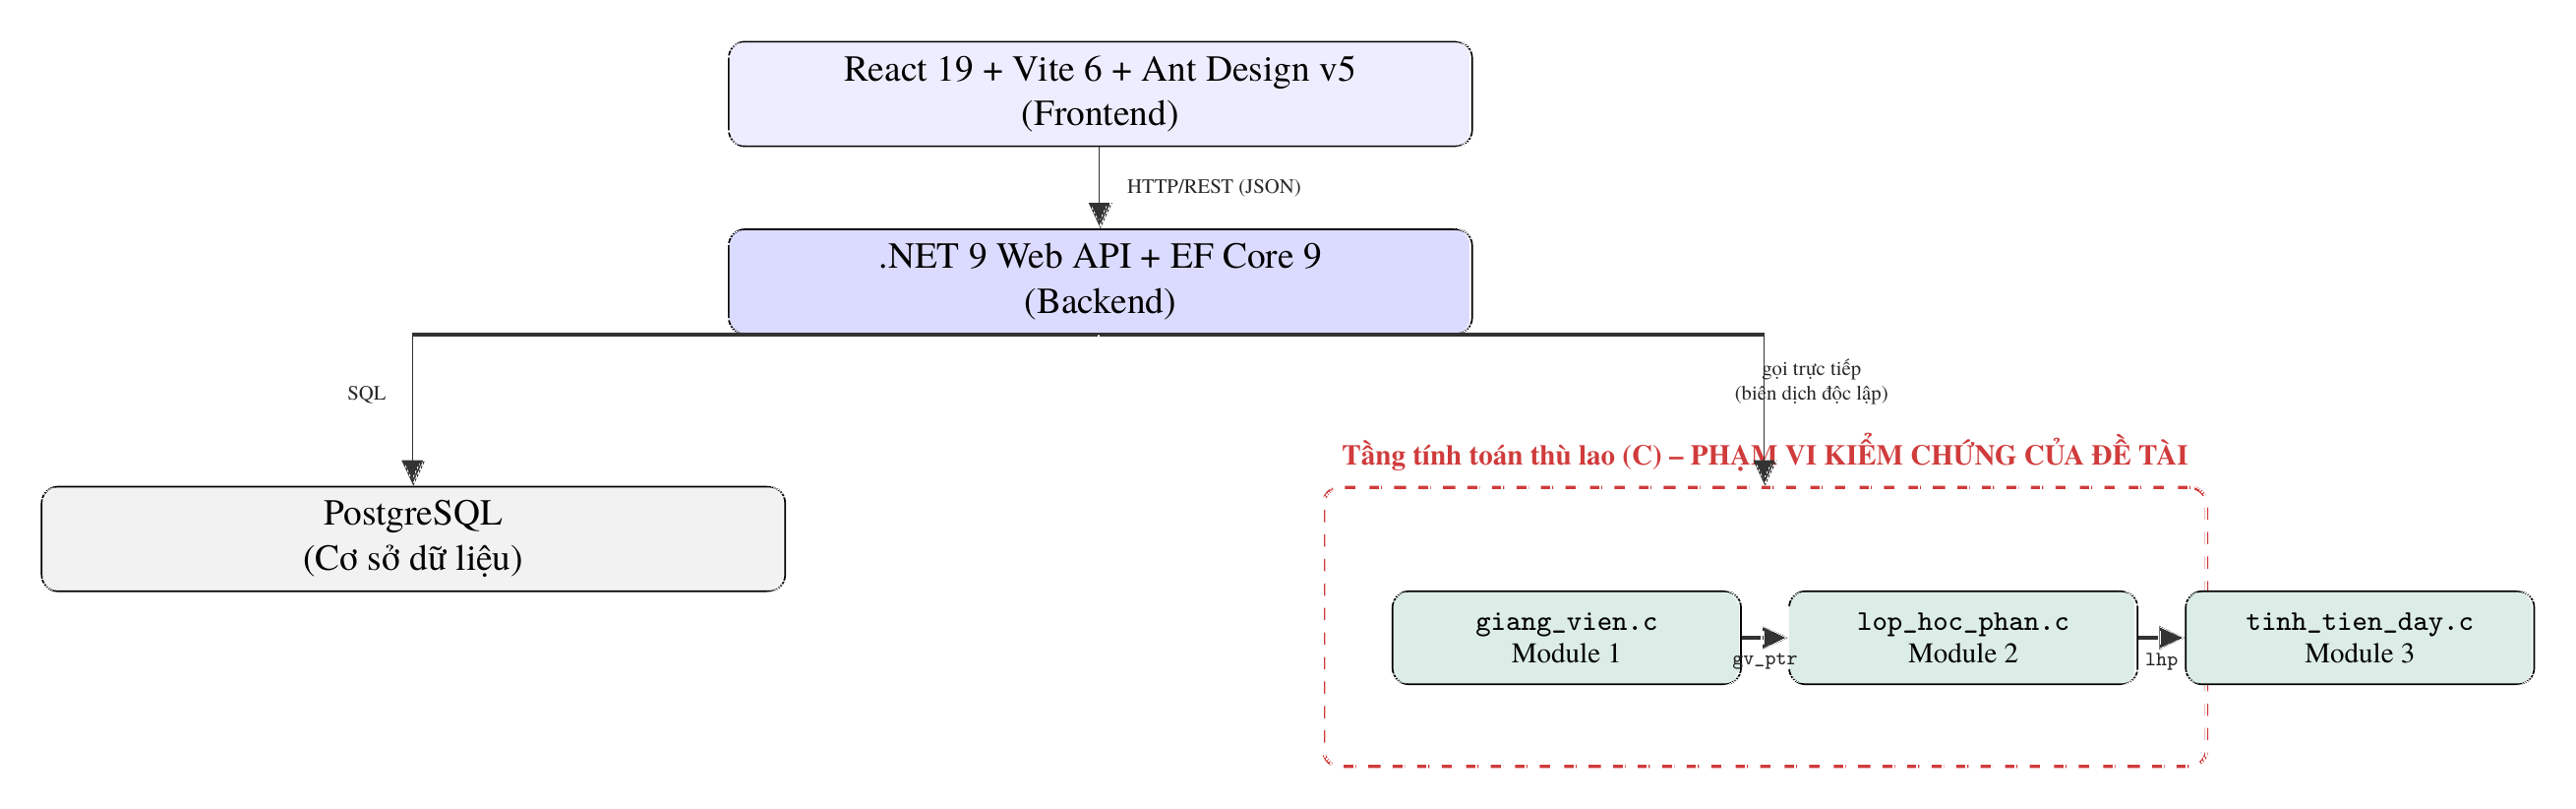
\includegraphics[width=\linewidth]{diagram6_e2e_architecture.png}
  \caption{Kiến trúc tổng quan DuongUniversity Management System -- tầng tính toán C (viền đỏ nét đứt) biên dịch độc lập với .NET, không được GC/bounds-checking của .NET bảo vệ}
  \label{fig:e2e-arch}
\end{figure}

\Cref{fig:e2e-arch} khớp đúng mô tả bằng chữ ở trên: request từ frontend đi qua backend .NET, backend rẽ 2 nhánh -- một sang PostgreSQL để đọc/ghi dữ liệu bền vững, một gọi trực tiếp vào tầng tính toán C (biên dịch thành thư viện/tiến trình riêng, không chạy trong runtime .NET) để tính thù lao; chính đường rẽ thứ hai này là ranh giới an toàn bị mất tác dụng của .NET, và là lý do 3 module C (viền đỏ) là đối tượng kiểm chứng duy nhất của đề tài.

\subsection{Mô tả 3 module mục tiêu}

\begin{itemize}
  \item \textbf{Module 1 -- Quản lý Giảng viên} (\texttt{giang\_vien.c}/\texttt{.h}): định nghĩa struct \texttt{GiangVien} (\texttt{id}, \texttt{maGiangVien}, \texttt{hoTen}, \texttt{bangCap}, \texttt{heSoBangCap}, \texttt{is\_deleted}) và cặp hàm \texttt{add\_lecturer\_VULN()}/\texttt{add\_lecturer\_SAFE()}, \texttt{delete\_lecturer\_VULN()}/\texttt{delete\_lecturer\_SAFE()}.
  \item \textbf{Module 2 -- Quản lý Lớp học phần} (\texttt{lop\_hoc\_phan.c}/\texttt{.h}): định nghĩa struct \texttt{LopHocPhan} (\texttt{id}, \texttt{maLop}, \texttt{soTiet}, \texttt{heSoHocPhan}, \texttt{soLuongSinhVien}, và đặc biệt \textbf{\texttt{gv\_ptr}} -- con trỏ thô trỏ sang \texttt{GiangVien}, chính là điểm liên kết xuyên module tạo ra rủi ro CWE-416/476) và cặp hàm \texttt{create\_class\_section\_VULN()}/\texttt{\_SAFE()}.
  \item \textbf{Module 3 -- Tính tiền dạy \& Thanh toán} (\texttt{tinh\_tien\_day.c}/\texttt{.h}): định nghĩa struct \texttt{Config} (\texttt{heSoQuyMoLop}, \texttt{dinhMucTienChuan}, \texttt{nam}) và 3 cặp hàm \texttt{calculate\_e2e\_salary\_VULN()}/\texttt{\_SAFE()}, \texttt{export\_report\_VULN()}/\texttt{\_SAFE()}, \texttt{pack\_class\_size\_byte\_VULN()}/\texttt{\_SAFE()} -- hàm cuối đóng gói \texttt{soLuongSinhVien} vào bản ghi audit log dạng \texttt{char}.
\end{itemize}

\noindent\textit{Lưu ý:} field \texttt{Config.heSoQuyMoLop} được \textbf{khai báo nhưng không hề được đọc} bởi \texttt{tinh\_tien\_day.c} -- hệ số quy mô lớp thật sự dùng trong công thức dưới đây được tính lại từ \texttt{soLuongSinhVien} (xem statement tường minh tại \Cref{sec:params}), không lấy từ field này. Đây là một field ``chết'' (dead field) phát hiện được khi đối chiếu lại công thức thật với mô hình Z3 ở Chương 3.

\Cref{lst:gvstruct,lst:lhpstruct} trích \emph{nguyên văn} định nghĩa 2 struct cốt lõi từ chính mã nguồn thật của đề tài -- trường \texttt{gv\_ptr} (con trỏ thô, không đếm tham chiếu) chính là điểm liên kết xuyên module tạo ra CWE-416/476 đã nêu.

\lstinputlisting[language=C,firstline=7,lastline=14,caption={Struct \texttt{GiangVien} -- trích nguyên văn \texttt{giang\_vien.h} (dòng 7--14)},label={lst:gvstruct}]{code/giang_vien.h}

\lstinputlisting[language=C,firstline=9,lastline=17,caption={Struct \texttt{LopHocPhan} -- trích nguyên văn \texttt{lop\_hoc\_phan.h} (dòng 9--17)},label={lst:lhpstruct}]{code/lop_hoc_phan.h}

Công thức tính tiền dạy gồm 2 bước, giữ nguyên 100\% giữa bản VULN và bản SAFE (chỉ khác kiểu dữ liệu):
\begin{align*}
  \text{heSoQuyMo} &= (\text{soLuongSinhVien} > 50)\ ?\ 0.2 : 0.0 \\
  \text{soTietQuyDoi} &= \text{soTiet} \times (\text{heSoHocPhan} + \text{heSoQuyMo}) \\
  \text{tienDay} &= \text{soTietQuyDoi} \times \text{gv\_ptr}.\text{heSoBangCap} \times \text{dinhMucTienChuan}
\end{align*}

\subsection{Sơ đồ quan hệ struct (ERD)}

\Cref{fig:erd} thể hiện quan hệ giữa 3 struct và các trường dữ liệu liên quan trực tiếp tới một CWE cụ thể (tô đỏ), đối lập với trường \texttt{dinhMucTienChuan} dùng kiểu \texttt{long long} (int64) đã được chứng minh an toàn (tô xanh, xem Check 2, \Cref{sec:ch3}).

\begin{figure}[H]
  \centering
  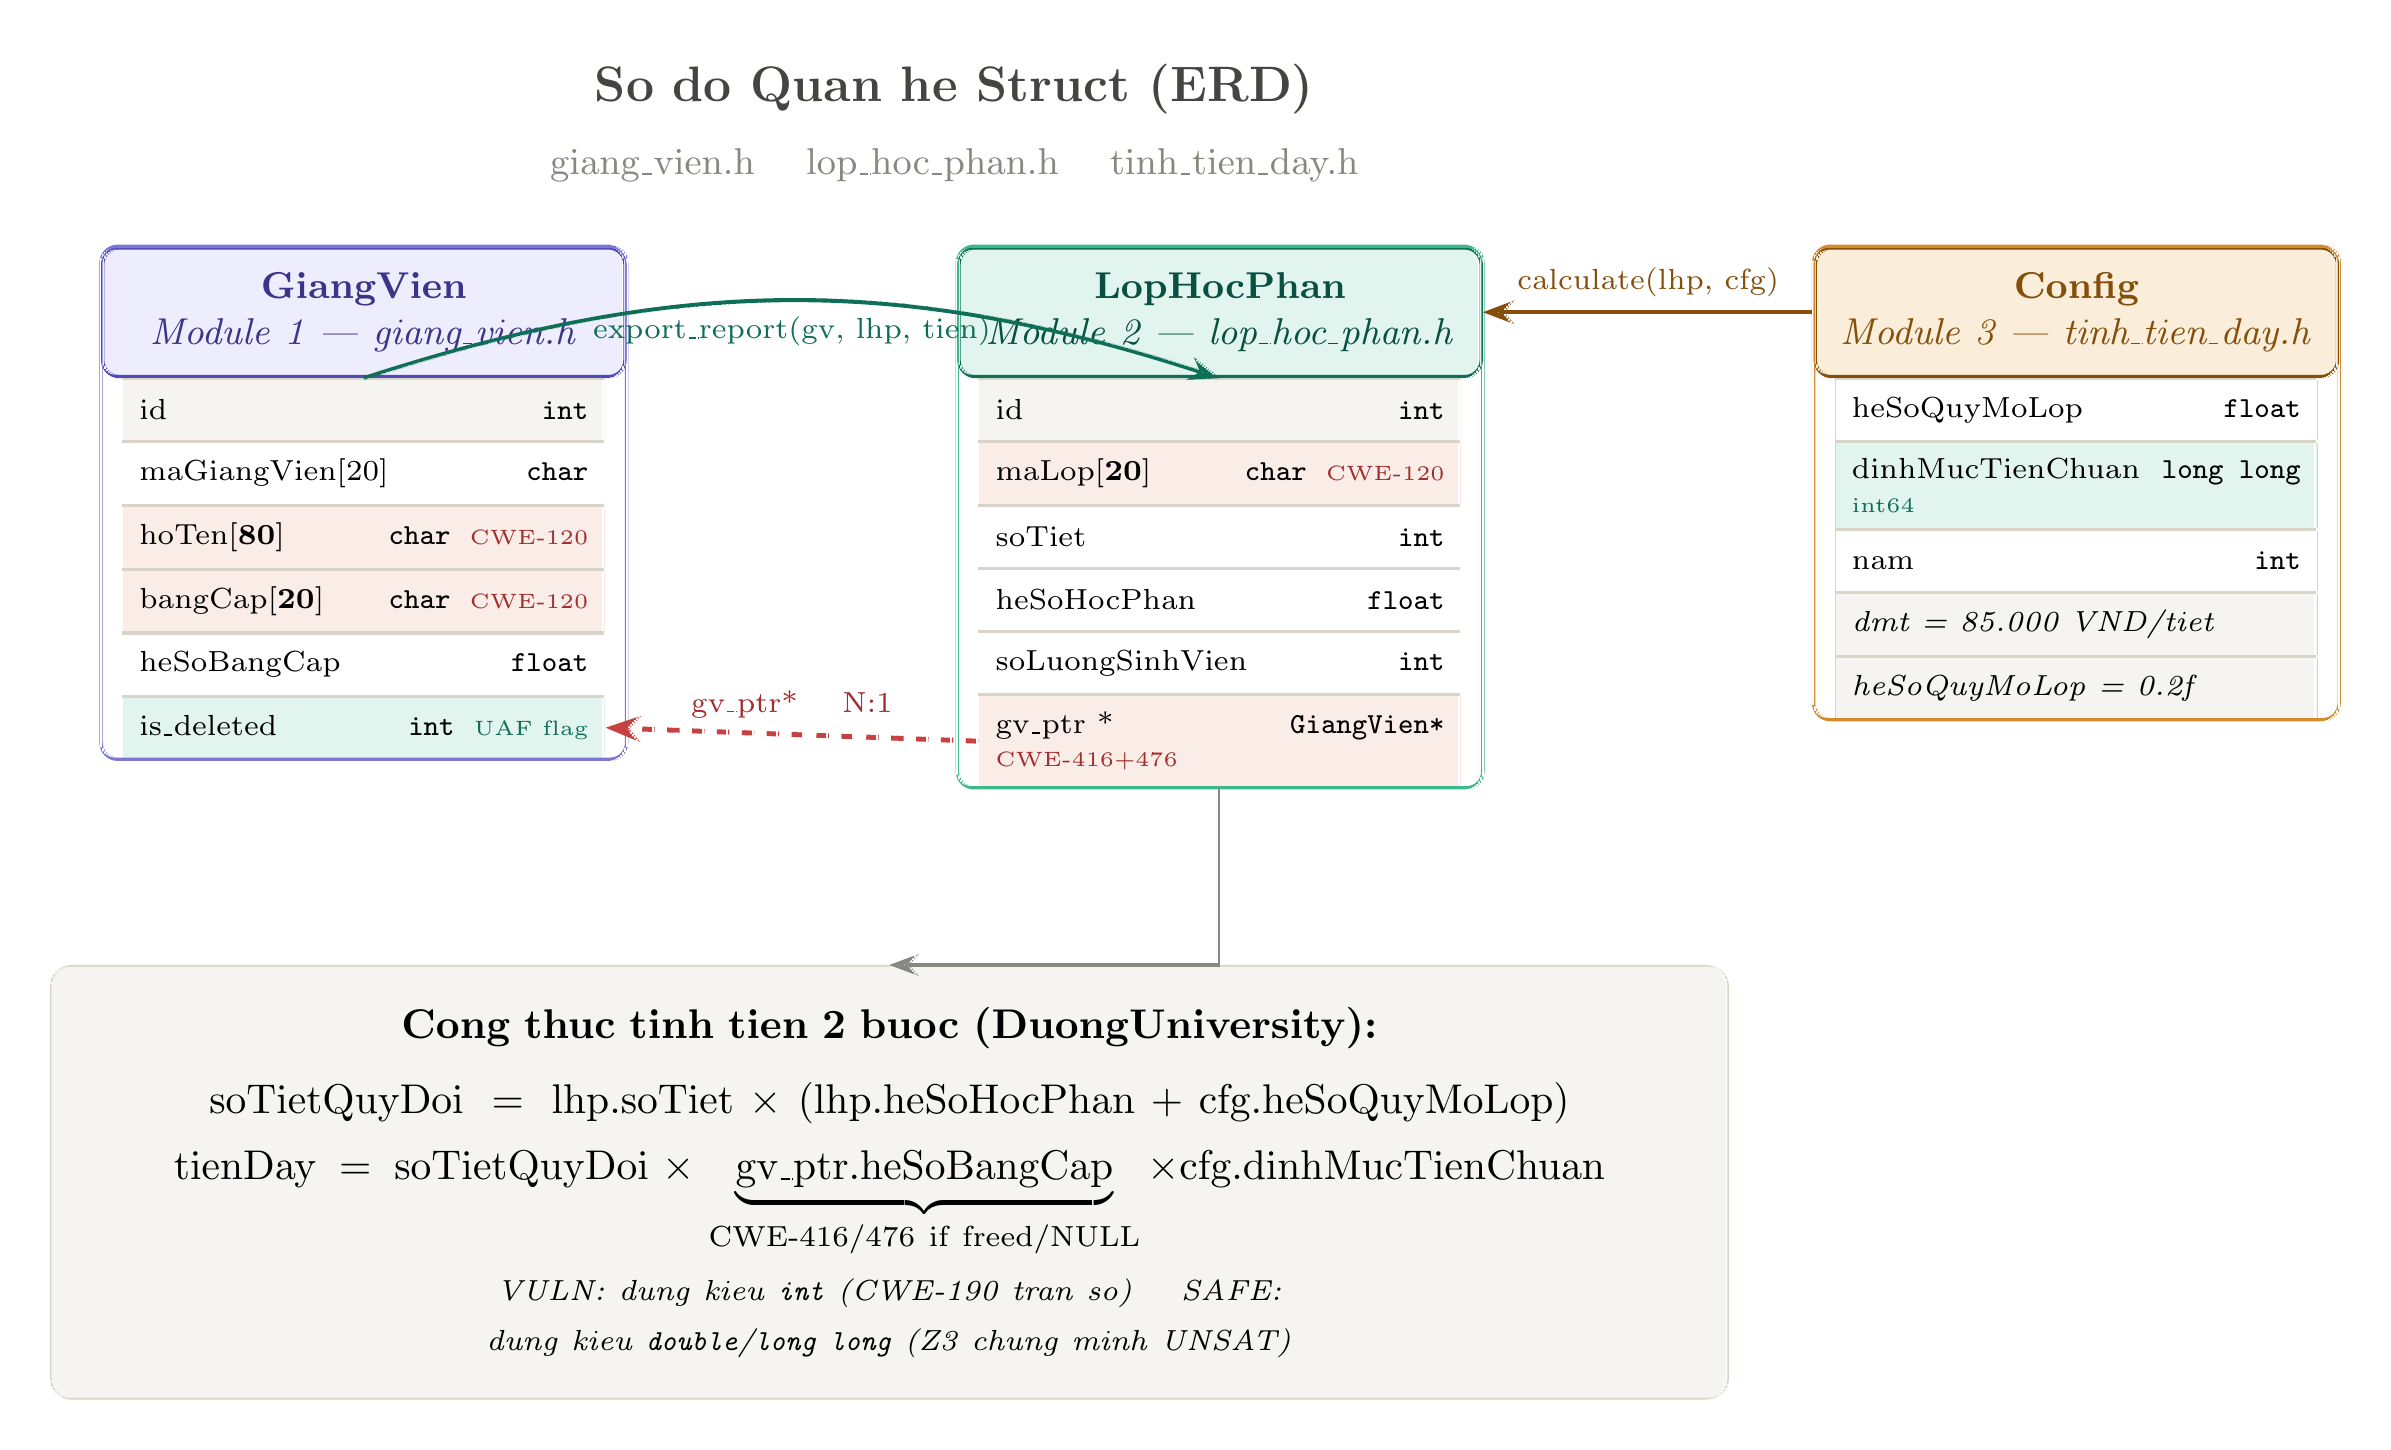
\includegraphics[width=0.95\linewidth]{diagram2_entity_relationship.png}
  \caption{Sơ đồ quan hệ 3 struct \texttt{GiangVien}, \texttt{LopHocPhan}, \texttt{Config} và các trường liên quan tới CWE-120/416/476/190}
  \label{fig:erd}
\end{figure}

\subsection{Sơ đồ luồng dữ liệu (DFD)}

\Cref{fig:dfd} theo dõi dữ liệu từ \texttt{stdin} (không tin cậy) qua Module 1, Module 2, tới Module 3, đánh dấu đúng vị trí mã nguồn (tên file, số dòng) nơi mỗi lỗ hổng CWE-120/416/190/476 phát sinh, cùng kết quả đối chứng của Chương 3 (Z3) và Chương 4 (fuzzing) ngay trên sơ đồ.

\begin{figure}[H]
  \centering
  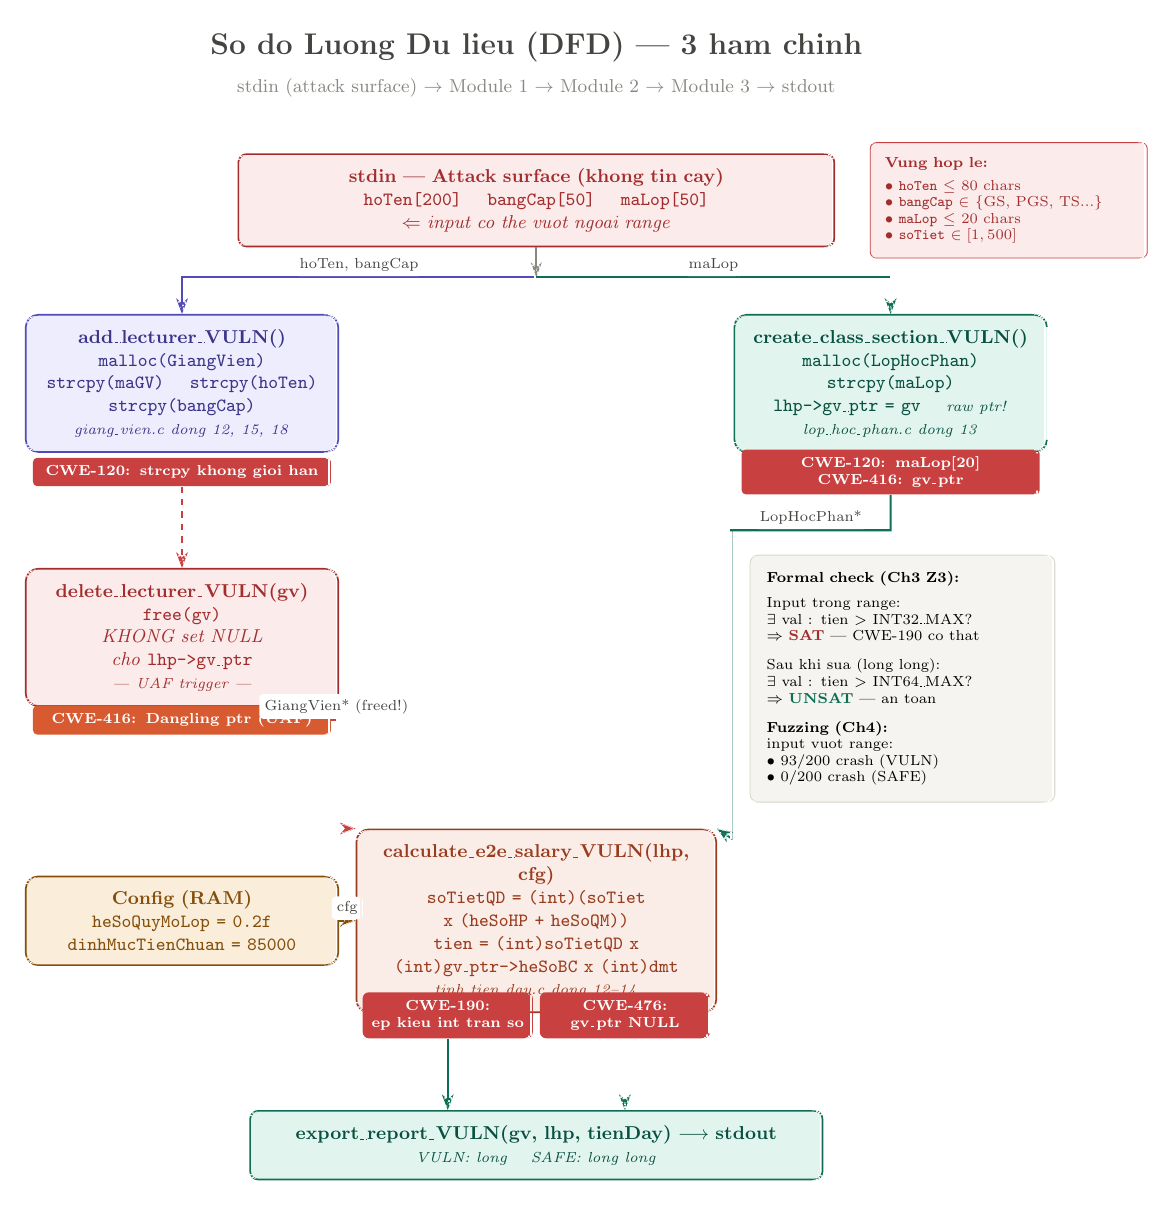
\includegraphics[width=\linewidth]{diagram3_data_flow.png}
  \caption{Sơ đồ luồng dữ liệu qua 3 hàm chính, đánh dấu vị trí phát sinh CWE và kết quả đối chứng Z3/fuzzing}
  \label{fig:dfd}
\end{figure}

\noindent\textit{Lưu ý:} Hai sơ đồ trên được dựng ở giai đoạn đầu của đề tài, khi hệ thống mới có 4 lỗ hổng CWE-120/416/190/476. Lỗ hổng thứ 5 (CWE-1288) và thứ 6 (CWE-197, cùng biến thể ``trùng lặp byte'' của nó) được bổ sung sau nên chưa xuất hiện trên hai hình trên -- được trình bày đầy đủ bằng sơ đồ trạng thái tại \Cref{sec:ch1} (nhãn \texttt{byte\_truncated}) và bảng kết quả tại \Cref{sec:ketqua}.

\subsection{Attack surface}

\begin{itemize}
  \item \texttt{stdin}: \texttt{hoTen} (buffer nhận 200 byte) được \texttt{strcpy} vào \texttt{hoTen[80]} không kiểm tra độ dài -- \textbf{CWE-120}.
  \item \texttt{bangCap} nhập từ \texttt{stdin} không được validate nghiêm ngặt ở bản VULN, rơi vào hệ số mặc định $1.0$ khi sai -- \textbf{CWE-1288}.
  \item \texttt{gv\_ptr} là con trỏ thô xuyên module, không có cơ chế đếm tham chiếu hay huỷ liên kết tự động khi \texttt{GiangVien} bị \texttt{free()} -- \textbf{CWE-416/CWE-476}.
  \item Phép nhân \texttt{soTietQuyDoi} $\times$ \texttt{heSoBangCap} $\times$ \texttt{dinhMucTienChuan} thực hiện trên kiểu \texttt{int} 32-bit ở bản VULN -- \textbf{CWE-190}.
  \item \texttt{soLuongSinhVien} (int, có thể tới vài trăm với lớp đại cương) bị ép kiểu xuống \texttt{char} không kiểm tra phạm vi khi đóng gói audit log -- \textbf{CWE-197}.
\end{itemize}

\subsection{Kích thước/độ phức tạp}

Hệ thống mục tiêu gồm \textbf{520 dòng mã C} (bao gồm cả header) chia trong \textbf{3 file module + 2 file driver} (\texttt{main.c} cho bản VULN, \texttt{main\_fixed.c} cho bản SAFE, dùng chung 3 module), với \textbf{12 hàm chính} (6 hàm \texttt{\_VULN} đối xứng 1-1 với 6 hàm \texttt{\_SAFE}), tạo điều kiện để mọi bản vá đều có thể so sánh trực tiếp hành vi trước/sau trên cùng một lời gọi hàm.

\section{Phương pháp Thực hiện}
\label{sec:phuongphap}

\subsection{Chương 1 -- Mô hình hóa Kripke \& Kiểm chứng BMC}
\label{sec:ch1}

\textbf{Module:} \texttt{ch1\_models/kripke\_bmc.py}.

Kripke structure $M = (S, S_0, R, L)$ được dựng với \textbf{6 trạng thái ở bản FIXED} ($S_0$ INIT $\to$ $S_1$ GV\_ASSIGNED $\to$ \{$S_{2A}$ CALC\_THUONG $\mid$ $S_{2B}$ CALC\_DONG\} $\to$ $S_3$ EXPORTED, và $S_4$ ERROR) và \textbf{7 trạng thái ở bản BUGGY} (thêm $S_5$ INVALID\_CALC -- đường tắt nhảy trực tiếp từ $S_0$ sang tính tiền, bỏ qua bước phân công giảng viên). \Cref{fig:kripke} minh họa sơ đồ chuyển trạng thái cùng kết quả BMC $P_1$--$P_4$ trên phiên bản gốc trước khi bổ sung $P_5$ và tách $S_{2A}$/$S_{2B}$ (xem giải thích dưới hình và bảng kết quả cập nhật đầy đủ tại \Cref{sec:ketqua}).

Hai trạng thái $S_{2A}$ CALC\_THUONG và $S_{2B}$ CALC\_DONG (thay cho 1 $S_2$ SALARY\_CALC duy nhất trước đây) mô hình hóa đúng nhánh rẽ \emph{thật} trong \texttt{tinh\_tien\_day.c}: \texttt{heSoQuyMo = (soLuongSinhVien > 50) ? 0.2 : 0.0} -- tức là kết hợp \textbf{2 tham số đầu vào} \texttt{soTiet} và \texttt{soLuongSinhVien} thành 1 tham số tổng hợp \texttt{soTietQuyDoi} \emph{tăng dần theo cả hai tham số} (xem chứng minh đơn điệu tại \Cref{sec:params}), và vì \emph{rất nhiều} giá trị \texttt{soLuongSinhVien} khác nhau ($0..50$ hoặc $51..300$) cùng rơi vào 1 trong 2 trạng thái này, mỗi trạng thái được gắn với đúng 1 \textbf{statement} (predicate) tường minh:
\begin{align*}
  S_{2A}\text{ CALC\_THUONG} &\equiv (0 \le \text{soLuongSinhVien} \le 50) \\
  S_{2B}\text{ CALC\_DONG} &\equiv (\text{soLuongSinhVien} > 50)
\end{align*}
Cả 2 nhánh đều mang nhãn \texttt{assigned}+\texttt{calculated} như nhau nên không làm thay đổi kết quả $P_1$--$P_5$ (đã xác nhận lại bằng cách chạy lại BMC sau khi sửa, xem \Cref{sec:ketqua}) -- việc tách trạng thái phục vụ tính \emph{truy vết tường minh} giữa mô hình điều khiển định tính (Kripke) và ràng buộc số học định lượng đã sửa ở Check 1/2 (Z3, \Cref{sec:ch3}), không phải để tạo thêm phát hiện lỗi mới.

\begin{figure}[H]
  \centering
  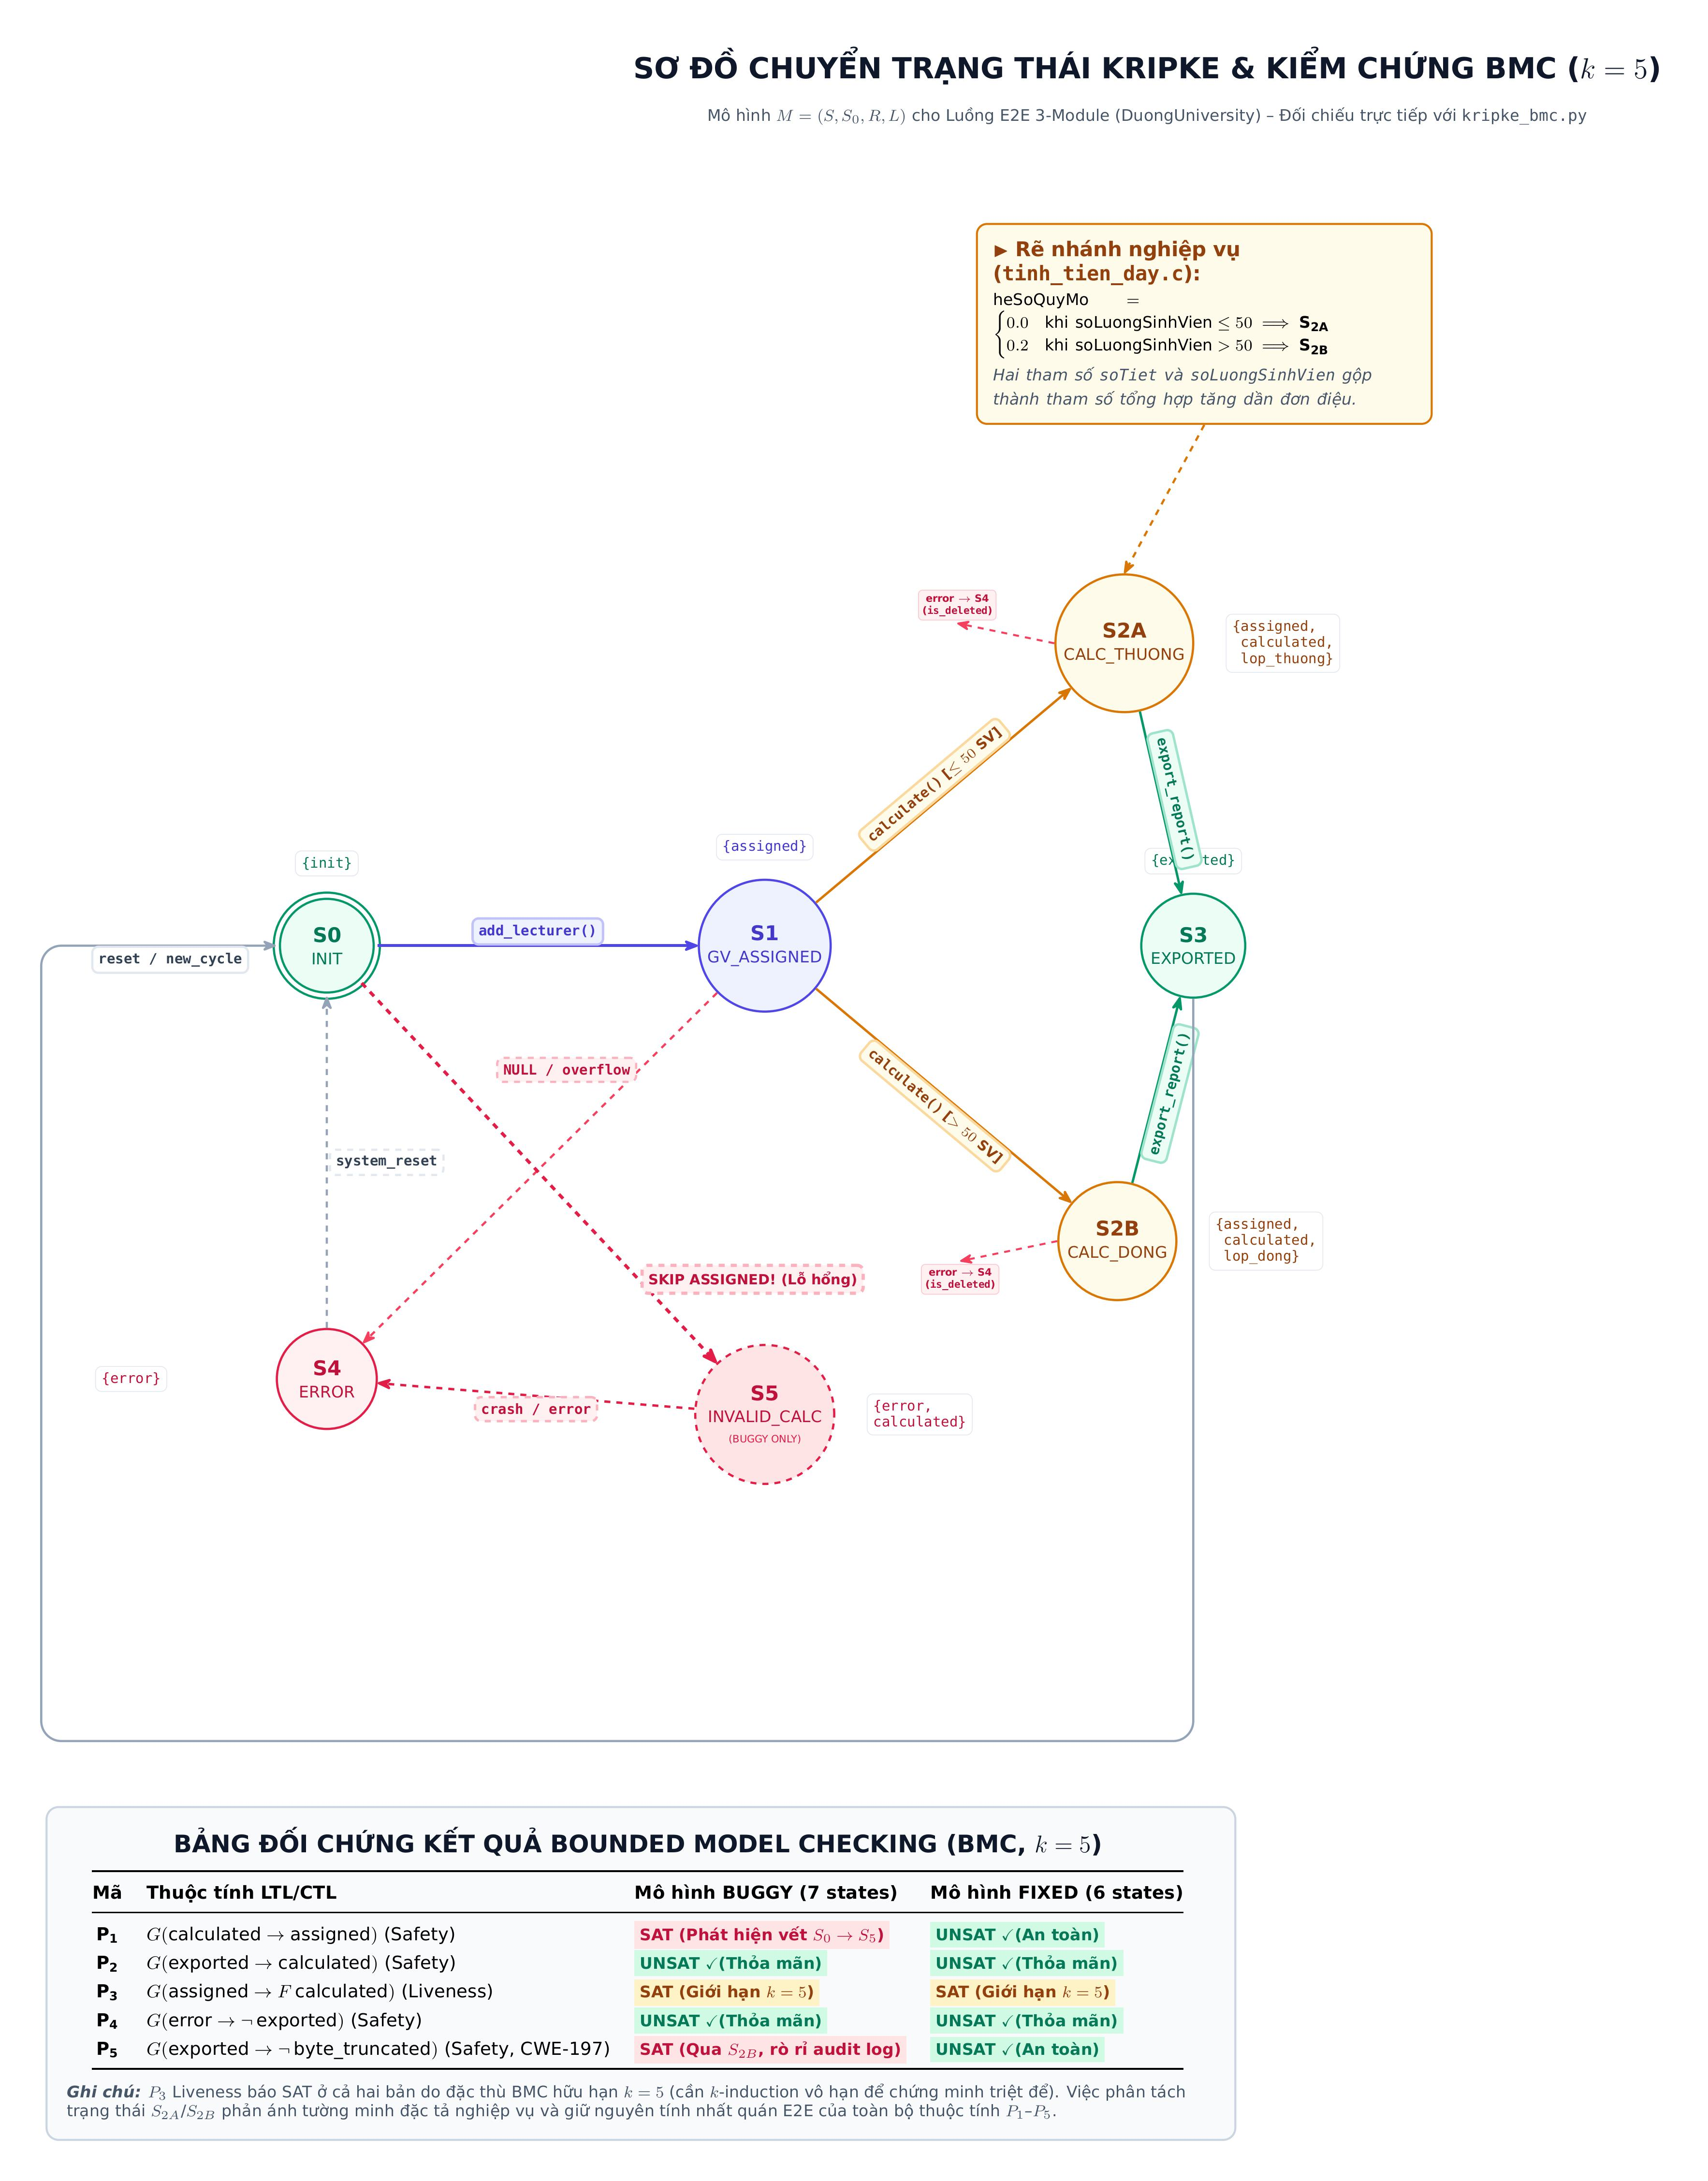
\includegraphics[width=\linewidth]{diagram1_state_transition_fixed.png}
  \caption{Sơ đồ chuyển trạng thái Kripke và kết quả BMC $k=5$ (thuộc tính $P_1$--$P_4$; hình vẽ ở phiên bản gốc trước khi bổ sung $P_5$ và tách $S_2$ thành $S_{2A}$/$S_{2B}$ -- xem văn bản và \Cref{sec:ketqua} để có mô hình và bảng kết quả đầy đủ, cập nhật)}
  \label{fig:kripke}
\end{figure}

\textbf{5 thuộc tính LTL/CTL} được kiểm chứng bằng BMC với $k=5$:
\begin{itemize}
  \item $P_1$ (Safety): $G(\text{calculated} \to \text{assigned})$ -- chưa phân công thì không được tính tiền.
  \item $P_2$ (Safety): $G(\text{exported} \to \text{calculated})$ -- chưa tính tiền thì không được xuất báo cáo.
  \item $P_3$ (Liveness): $G(\text{assigned} \to F\,\text{calculated})$ -- đã phân công thì cuối cùng phải tính tiền.
  \item $P_4$ (Safety): $G(\text{error} \to \lnot\,\text{exported})$ -- hệ thống lỗi thì không được xuất báo cáo.
  \item $P_5$ (Safety, bổ sung cho CWE-197): $G(\text{exported} \to \lnot\,\text{byte\_truncated})$ -- báo cáo xuất ra không được mang dữ liệu ép kiểu sai lệch.
\end{itemize}

Hàm \texttt{cross\_validate\_with\_pattern\_scanner()} gọi lại chính \texttt{pattern\_scanner.py} của Chương 2 để tự động xác nhận trạng thái lỗi $S_4$/$S_3$\_EXPORTED\_TRUNCATED trong mô hình Kripke trừu tượng khớp với đúng vị trí lỗ hổng thật trên mã nguồn C -- liên kết Chương 1 $\leftrightarrow$ Chương 2, tránh việc mô hình hình thức tồn tại độc lập, tách rời code thật.

\subsection{Chương 2 -- Kiểm toán an toàn bộ nhớ}
\label{sec:ch2}

\textbf{Module:} \texttt{ch2\_memsafe/pattern\_scanner.py}.

Công cụ quét trực tiếp mã nguồn C dạng văn bản (regex/so khớp chuỗi, không phải phân tích AST/data-flow đầy đủ) trên 3 file \texttt{giang\_vien.c}, \texttt{lop\_hoc\_phan.c}, \texttt{tinh\_tien\_day.c} và driver \texttt{main\_fixed.c}, với 5 quy tắc phát hiện: \texttt{strcpy} (CWE-120), \texttt{dangling\_free} (CWE-416), \texttt{unchecked\_nested\_deref} (CWE-476), \texttt{int\_overflow\_cast} (CWE-190), \texttt{unchecked\_numeric\_truncation} (CWE-197). Phạm vi tìm ``đã được bảo vệ'' (guard-check) được scope đúng theo \emph{hàm bao quanh} thay vì cửa sổ N dòng cố định, tránh bỏ sót guard nằm xa vị trí truy cập trong hàm dài.

\textbf{Bổ sung bằng chứng động (\texttt{memory\_trace\_demo.py}):} phân tích tĩnh không thể trả lời câu hỏi ``bộ nhớ thực sự được dùng ra sao khi chương trình chạy''. Script này biên dịch cùng một luồng E2E 7 bước bằng 2 trình biên dịch: \textbf{Plain GCC} (chỉ in địa chỉ con trỏ thật, không phát hiện lỗi) và \textbf{Clang64 + AddressSanitizer thật}~\cite{clangasan} (công cụ độc lập tự phát hiện \texttt{heap-use-after-free}), cho phép đối chiếu hành vi ``im lặng'' (nguy hiểm) và hành vi ``bị công cụ chặn'' trên cùng một lỗi.

\subsection{Chương 3 -- Kiểm chứng hình thức SMT/Z3}
\label{sec:ch3}

\textbf{Module:} \texttt{ch3\_staticsat/smt\_verify.py}.

Khác với test thông thường (thử một vài input), Z3 SMT solver~\cite{demoura2008z3} chứng minh một mệnh đề đúng/sai trên \emph{toàn miền giá trị hợp lệ} cùng lúc, với 7 phép kiểm chứng:

\begin{itemize}
  \item \textbf{Check 1}: $\exists$ input hợp lệ ($\text{numClasses}\in[1,20]$, $\text{soTiet}\in[15,120]$, $\text{soLuongSinhVien}\in[0,300]$,\dots) : $\text{tienDay} > \text{INT32\_MAX}$? $\Rightarrow$ \textbf{SAT} -- CWE-190 có thật.
  \item \textbf{Check 2}: cùng câu hỏi với ngưỡng \texttt{INT64\_MAX} trên kiểu \texttt{long long} $\Rightarrow$ \textbf{UNSAT} -- an toàn tuyệt đối.
  \item \textbf{Check 3}: $\text{gv\_ptr} = \text{NULL} \lor \text{is\_deleted} \to \text{tienDay} = 0$? -- mô hình hóa bằng \emph{đúng công thức thật} trong \texttt{calculate\_e2e\_salary\_SAFE()} $\Rightarrow$ \textbf{UNSAT} -- guard hoạt động đúng.
  \item \textbf{Check 4}: $\exists\, \text{soLuongSinhVien}\in[0,300]$ : ép kiểu \texttt{(char)} (mô phỏng bằng số học modulo 256) cho giá trị khác giá trị gốc? $\Rightarrow$ \textbf{SAT} -- phản ví dụ $128 \to -128$.
  \item \textbf{Check 5}: cùng câu hỏi nhưng với guard $0 \le n \le 127$ đứng trước $\Rightarrow$ \textbf{UNSAT} -- chứng minh bản vá loại trừ hoàn toàn CWE-197.
  \item \textbf{Check 6}: $\exists\, a \ne b \in [0,300]$ : ép kiểu cho ra cùng 1 byte? $\Rightarrow$ \textbf{SAT} -- phản ví dụ $a=0, b=256$ cùng cho byte $=0$ (lớp nguy hiểm nhất: 2 lớp học hoàn toàn khác nhau bị nhầm thành một).
  \item \textbf{Check 7} (mới, CWE-1288): $\exists$ 2 danh mục \texttt{bangCap} khác nhau (\texttt{CU\_NHAN} thật, và 1 chuỗi không hợp lệ) : cho cùng 1 \texttt{heSoBangCap}? $\Rightarrow$ \textbf{SAT} -- cả hai cùng rơi vào nhánh fallback $1.0$ của if-chain thật trong \texttt{add\_lecturer\_*()} (xem statement đầy đủ tại \Cref{sec:quytrinh}).
\end{itemize}

Các ràng buộc nghiệp vụ dùng đúng con số đã đặc tả tại \Cref{tab:range} ($\text{soTiet}\in[1,500]$, $\text{dinhMucTienChuan}\in[50\,000,200\,000]$ VNĐ).

\textbf{Một lỗi mô hình đã được tìm và sửa ở Check 1/2:} bản gốc mô hình hóa hệ số quy mô lớp bằng 1 biến \texttt{Real} \emph{tự do} \texttt{heSoQuyMoLop} $\in[0.1,0.5]$/$[0.1,2.0]$, đặt tên theo field \texttt{Config.heSoQuyMoLop} (\texttt{tinh\_tien\_day.h:8}) -- nhưng field này \textbf{không bao giờ được code C thật đọc} (\texttt{tinh\_tien\_day.c} không có \texttt{cfg->heSoQuyMoLop} ở đâu cả, xem đối chiếu tại \Cref{sec:params}), nên phần chứng minh trước đây không phản ánh đúng công thức chạy thực tế. Đã sửa bằng cách thêm \texttt{soLuongSinhVien} là biến Z3 thật và định nghĩa \texttt{heSoQuyMo = If(soLuongSinhVien > 50, 0.2, 0.0)} -- đúng \emph{statement} thật trong code, không phải biến tự do. Sau khi sửa, Check 1 vẫn \textbf{SAT} và Check 2 vẫn \textbf{UNSAT} (kết luận định tính không đổi), nhưng phản ví dụ của Check 1 nay là bộ giá trị mà mô hình sửa vẫn có thể thật sự sinh ra từ code, xem số liệu cập nhật tại \Cref{sec:ketqua}.

\subsection{Chương 4 -- Dynamic Fuzzing}
\label{sec:ch4}

\textbf{Module:} \texttt{ch4\_dynafuzz/fuzzer\_blackbox.py} và \texttt{fuzzer\_whitebox.py}.

\textbf{Black-box}: sinh 200 input ngẫu nhiên (tên/bằng cấp/mã lớp qua \texttt{stdin}), đo crash rate thật trên \texttt{salary\_calc.exe} (VULN) đối chứng \texttt{salary\_calc\_fixed.exe} (SAFE). Riêng CWE-197 được fuzz qua subcommand \texttt{e2e\_byte\_truncate <n>} với 2 chiến lược: (a) 200 giá trị ngẫu nhiên trong $[-50,400]$, và (b) \textbf{Boundary Value Analysis} -- 17 giá trị biên \emph{thiết kế sẵn} (quanh mép \texttt{char} $\{-129,\dots,129\}$, quanh mép chu kỳ 256 $\{-256,\dots,257\}$, và giá trị lớp đại cương $\{300,384\}$) chạy tất định thay vì phó mặc ngẫu nhiên -- đảm bảo luôn phát hiện được lớp lỗi nguy hiểm nhất (trùng lặp byte).

\textbf{White-box (Z3-guided)}: giải trực tiếp 7 ràng buộc Z3 tương ứng 6 lỗ hổng CWE đã biết trước (không phải symbolic execution duyệt CFG tự động) -- hằng số \texttt{MAX\_NAME}/\texttt{MAX\_MALOP} được đọc trực tiếp từ header \texttt{.h} qua \texttt{read\_header\_define()} thay vì hard-code, nên ràng buộc Z3 tự động bám theo đúng source hiện tại nếu hằng số đổi.

\section{Kết quả và Phân tích}
\label{sec:ketqua}

Toàn bộ số liệu trong mục này trích xuất verbatim từ log thực thi tự động lưu tại \texttt{btl\_softsec/logs/} (sinh bởi \texttt{python run\_all.py}), không phải số liệu minh họa.

\subsection{Kết quả Chương 1 -- BMC}

\begin{table}[H]
  \centering
  \caption{Kết quả BMC $k=5$ trên 5 thuộc tính $P_1$--$P_5$}
  \label{tab:bmc}
  \small
  \begin{tabularx}{\linewidth}{@{}l X >{\centering\arraybackslash}p{2.6cm} >{\centering\arraybackslash}p{1.7cm}@{}}
    \toprule
    \textbf{Thuộc tính} & \textbf{Công thức} & \textbf{BUGGY} & \textbf{FIXED} \\
    \midrule
    $P_1$ Safety   & $G(\text{calculated}\to\text{assigned})$          & \textbf{SAT} -- counterexample qua $S_5$ (chi tiết dưới bảng) & \textbf{UNSAT} \checkmark \\
    $P_2$ Safety   & $G(\text{exported}\to\text{calculated})$          & \textbf{UNSAT} \checkmark & \textbf{UNSAT} \checkmark \\
    $P_3$ Liveness & $G(\text{assigned}\to F\,\text{calculated})$      & \textbf{SAT} ($k{=}5$ limit) & \textbf{SAT} ($k{=}5$ limit) \\
    $P_4$ Safety   & $G(\text{error}\to\lnot\,\text{exported})$        & \textbf{UNSAT} \checkmark & \textbf{UNSAT} \checkmark \\
    $P_5$ Safety   & $G(\text{exported}\to\lnot\,\text{byte\_truncated})$ & \textbf{SAT} -- qua $S_{2B}$ (chi tiết dưới bảng) & \textbf{UNSAT} \checkmark \\
    \bottomrule
  \end{tabularx}
\end{table}

Mô hình FIXED hiện có \textbf{6 trạng thái} ($S_0,S_1,S_{2A},S_{2B},S_3,S_4$) và bản BUGGY có \textbf{7 trạng thái} (thêm $S_5$) -- xem \Cref{sec:ch1} để biết vì sao $S_2$ SALARY\_CALC gốc được tách thành $S_{2A}$/$S_{2B}$. Việc tách này không làm đổi bất kỳ kết quả SAT/UNSAT nào ở trên so với mô hình gốc (đã xác nhận bằng cách chạy lại BMC sau khi sửa).

\textbf{Counterexample trace thật} cho $P_1$ trên bản BUGGY (\texttt{logs/kripke\_bmc.log}):
\begin{quote}\ttfamily\footnotesize
Step 0: S0\_INIT [init] $\to$ Step 1: S5\_INVALID\_CALC [calculated,error] $\to$ Step 2: S4\_ERROR [error] \\
$\to$ Step 3: S0\_INIT [init] $\to$ Step 4: S1\_GV\_ASSIGNED [assigned] \\
$\to$ Step 5: S2A\_CALC\_THUONG [assigned,calculated,lop\_thuong]
\end{quote}

\textbf{Counterexample trace thật} cho $P_5$ trên bản BUGGY (\texttt{logs/kripke\_bmc.log}) -- nay đi qua đúng nhánh $S_{2B}$ CALC\_DONG (lớp đông, statement \Cref{sec:params}):
\begin{quote}\ttfamily\footnotesize
Step 0: S0\_INIT [init] $\to$ Step 1: S1\_GV\_ASSIGNED [assigned] $\to$ Step 2: S2B\_CALC\_DONG [assigned,calculated,lop\_dong] \\
$\to$ Step 3: S3\_EXPORTED [assigned,byte\_truncated,calculated,exported] \\
$\to$ Step 4: S0\_INIT [init] $\to$ Step 5: S1\_GV\_ASSIGNED [assigned]
\end{quote}

$P_3$ ra \textbf{SAT} ở cả 2 bản -- đây \emph{không phải lỗi mã nguồn}, mà là giới hạn kỹ thuật tự nhiên của BMC hữu hạn $k=5$ đối với thuộc tính Liveness (cần $k$-induction hoặc Büchi automata để chứng minh liveness vô hạn triệt để).

\subsection{Kết quả Chương 2 -- 9 findings}

\begin{table}[H]
  \centering
  \caption{Toàn bộ 9 cảnh báo phát hiện bởi \texttt{pattern\_scanner.py} trên code VULN; \texttt{main\_fixed.c} sạch tuyệt đối (0 finding)}
  \label{tab:findings}
  \small
  \begin{tabularx}{\linewidth}{@{}l l l X@{}}
    \toprule
    \textbf{Vị trí} & \textbf{CWE} & \textbf{Rule} & \textbf{Mức độ} \\
    \midrule
    \texttt{giang\_vien.c:12}     & CWE-120 & \texttt{strcpy}                    & HIGH \\
    \texttt{giang\_vien.c:15}     & CWE-120 & \texttt{strcpy} (\texttt{hoTen})    & HIGH \\
    \texttt{giang\_vien.c:18}     & CWE-120 & \texttt{strcpy} (\texttt{bangCap})  & HIGH \\
    \texttt{giang\_vien.c:35}     & CWE-416 & \texttt{dangling\_free}             & HIGH \\
    \texttt{lop\_hoc\_phan.c:13}  & CWE-120 & \texttt{strcpy} (\texttt{maLop})    & HIGH \\
    \texttt{tinh\_tien\_day.c:12} & CWE-190 & \texttt{int\_overflow\_cast}        & HIGH \\
    \texttt{tinh\_tien\_day.c:13} & CWE-190 & \texttt{int\_overflow\_cast}        & HIGH \\
    \texttt{tinh\_tien\_day.c:13} & CWE-476 & \texttt{unchecked\_nested\_deref}   & HIGH \\
    \texttt{tinh\_tien\_day.c:68} & CWE-197 & \texttt{unchecked\_numeric\_truncation} & HIGH \\
    \bottomrule
  \end{tabularx}
\end{table}

Điểm đáng chú ý: \texttt{pack\_class\_size\_byte\_SAFE()} nằm \emph{trong cùng file} \texttt{tinh\_tien\_day.c} với hàm VULN nhưng \textbf{không} bị báo động giả, vì scanner tìm thấy đúng guard \texttt{if (soLuongSinhVien < 0 || > 127)} trong phạm vi hàm bao quanh -- xác nhận cơ chế xét theo hàm (không phải theo tên file) hoạt động đúng.

\Cref{lst:delvuln,lst:delsafe} trích nguyên văn cặp hàm gây ra và khắc phục CWE-416 (dòng \texttt{giang\_vien.c:35} trong \Cref{tab:findings}): bản VULN \texttt{free(gv)} mà không huỷ liên kết \texttt{gv\_ptr} ở Module 2; bản SAFE nhận tham số \texttt{GiangVien **} để có thể tự đặt con trỏ gốc về \texttt{NULL} ngay sau khi giải phóng.

\lstinputlisting[language=C,firstline=32,lastline=37,caption={\texttt{delete\_lecturer\_VULN()} -- CWE-416: \texttt{free()} không huỷ liên kết},label={lst:delvuln}]{code/giang_vien.c}

\lstinputlisting[language=C,firstline=71,lastline=77,caption={\texttt{delete\_lecturer\_SAFE()} -- khắc phục: nhận \texttt{GiangVien **} để nullify con trỏ gốc},label={lst:delsafe}]{code/giang_vien.c}

\Cref{lst:packvuln,lst:packsafe} trích nguyên văn cặp hàm CWE-197 (dòng \texttt{tinh\_tien\_day.c:68} trong \Cref{tab:findings}), đúng cặp hàm được chứng minh hình thức ở Check 4/5 (\Cref{sec:ch3}).

\lstinputlisting[language=C,firstline=67,lastline=69,caption={\texttt{pack\_class\_size\_byte\_VULN()} -- CWE-197: ép kiểu không kiểm tra phạm vi},label={lst:packvuln}]{code/tinh_tien_day.c}

\lstinputlisting[language=C,firstline=75,lastline=82,caption={\texttt{pack\_class\_size\_byte\_SAFE()} -- khắc phục: guard \texttt{[0,127]} trước khi ép kiểu},label={lst:packsafe}]{code/tinh_tien_day.c}

\subsection{Kết quả kiểm chứng NFR-1/NFR-2 (\texttt{nfr\_check.py})}

Bổ sung cho \Cref{tab:nfr}: subcommand \texttt{e2e\_nfr\_bench} (mới thêm vào \texttt{main.c}/\texttt{main\_fixed.c}) đo \emph{thực nghiệm} 2 yêu cầu phi chức năng quan trọng nhất, chạy $N=10\,000$ lần trên chính 2 binary đã biên dịch của Chương 2 (không phải microbenchmark tách biệt):

\begin{itemize}
  \item \textbf{NFR-1 (Hiệu năng)}: trung bình $0{,}000014\,$ms/lần gọi \texttt{calculate\_\allowbreak e2e\_\allowbreak salary\_\allowbreak SAFE()} ($0{,}000011\,$ms/lần trên bản VULN) -- thấp hơn ngưỡng $10\,$ms gần $6$ bậc độ lớn -- \textbf{PASS}.
  \item \textbf{NFR-2 (Ổn định bộ nhớ)}: sau $10\,000$ lần tạo/xoá \texttt{GiangVien}+\texttt{LopHocPhan} liên tục, \texttt{WorkingSetSize} (đo qua \texttt{GetProcessMemoryInfo}) chỉ trôi $4$\,KB trên cả bản SAFE và bản VULN (ngưỡng $1024$\,KB) -- \textbf{PASS cả 2 bản}. Kết quả này \emph{nhất quán với lý thuyết} nêu ở \Cref{sec:thaoluan}: CWE-416 trong đề tài là lỗi con trỏ treo (dangling pointer, \texttt{gv\_ptr} vẫn trỏ tới vùng nhớ đã \texttt{free()}), không phải rò rỉ bộ nhớ (memory leak) -- cả \texttt{delete\_lecturer\_VULN()} lẫn \texttt{delete\_lecturer\_SAFE()} đều gọi \texttt{free()} đầy đủ, nên không có gì để rò rỉ; hai lớp lỗi bộ nhớ này độc lập với nhau.
\end{itemize}

Toàn bộ số liệu trích \emph{verbatim} từ \texttt{logs/nfr\_check.log} -- trước khi có subcommand này, NFR-1/NFR-2 chỉ được biện luận gián tiếp (công thức $O(1)$, 0/200 crash), chưa có phép đo trực tiếp ở đúng quy mô $10^4$ đã đặc tả.

\subsection{Kết quả Chương 3 -- SMT}

\begin{itemize}
  \item \textbf{Check 1 SAT}: counterexample $\text{numClasses}=20$, $\text{soTiet}=120$, $\text{soLuongSinhVien}=0$ (nên $\text{heSoQuyMo}=0.0$, đúng statement \Cref{sec:params}), $\text{heSoHocPhan}\approx 3.0$, $\text{heSoBangCap}\approx 2.0$, $\text{dinhMucTienChuan}=149\,131$ VNĐ $\Rightarrow$ tổng thù lao vượt \texttt{INT32\_MAX}. (Đã sửa mô hình để dùng đúng \texttt{soLuongSinhVien} thật thay cho biến tự do \texttt{heSoQuyMoLop} không tồn tại trong code -- xem \Cref{sec:params}; kết luận SAT không đổi.)
  \item \textbf{Check 2 UNSAT}: chứng minh \texttt{long long} an toàn tuyệt đối trong toàn bộ ràng buộc doanh nghiệp ($\text{numClasses}\in[1,100]$, $\text{dinhMucTienChuan}$ tới 2 triệu VNĐ).
  \item \textbf{Check 3 UNSAT}: guard-check (\texttt{gv\_ptr} NULL/đã xóa $\to$ lương $=0$) hoạt động đúng trên chính công thức thật.
  \item \textbf{Check 4 SAT}: phản ví dụ $\text{soLuongSinhVien}=128 \to \text{byte}=-128$.
  \item \textbf{Check 5 UNSAT}: với guard $[0,127]$ đúng trước, ép kiểu không bao giờ sai lệch.
  \item \textbf{Check 6 SAT}: $a=0$ (lớp rỗng thật) và $b=256$ (lớp có thật 256 sinh viên) đều cho byte $=0$ -- 2 tình huống nghiệp vụ hoàn toàn khác nhau không thể phân biệt sau khi xuất báo cáo.
  \item \textbf{Check 7 SAT} (mới, CWE-1288): giảng viên \texttt{CU\_NHAN} thật và 1 chuỗi \texttt{bangCap} không hợp lệ đều cho $\text{heSoBangCap}=1.0$ -- cùng lớp lỗi ``va chạm trạng thái'' như Check 6, nhưng ở Module 1 (xem \Cref{sec:quytrinh}); khác CWE-197, lỗi này không thể loại trừ hoàn toàn bằng cách từ chối (nghiệp vụ cần 1 giá trị fallback thật), bản SAFE chỉ thêm được cảnh báo phát hiện.
\end{itemize}

\subsection{Kết quả Chương 4 -- Fuzzing}

\begin{table}[H]
  \centering
  \caption{So sánh Black-box vs. White-box (lần chạy đại diện, \texttt{logs/fuzzer\_black/whitebox.log})}
  \label{tab:fuzz}
  \small
  \begin{tabular}{@{}l c c@{}}
    \toprule
    \textbf{Tiêu chí} & \textbf{Black-box} & \textbf{White-box (Z3)} \\
    \midrule
    Số lần thử                & 200 (ngẫu nhiên)      & 7 (giải trực tiếp) \\
    Số crash phát hiện (VULN) & 72/200 (36.0\%)       & 7/7 target (100\%) \\
    Số crash (SAFE)           & 0/200                 & -- \\
    Thời gian thực thi        & 9.86 s                & 0.3412 s \\
    Tốc độ tăng tốc           & mức cơ sở             & $\approx 28.9\times$ nhanh hơn \\
    \bottomrule
  \end{tabular}
\end{table}

\begin{figure}[H]
  \centering
  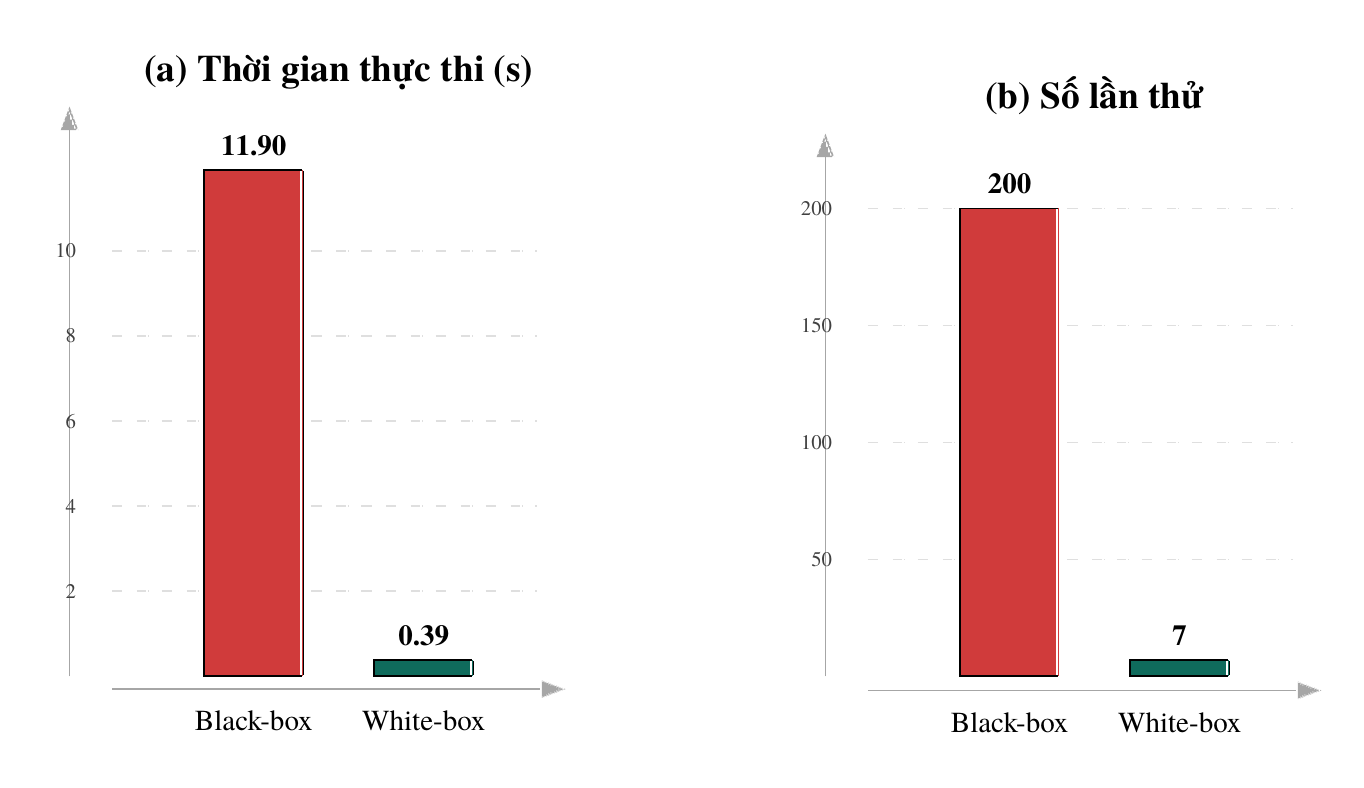
\includegraphics[width=\linewidth]{diagram5_fuzz_compare.png}
  \caption{Black-box vs. White-box: (a) thời gian thực thi và (b) số lần thử cần để phát hiện đủ lỗ hổng đã biết (số liệu khớp \protect\Cref{tab:fuzz})}
  \label{fig:fuzz-bar}
\end{figure}

Hai biểu đồ trên cùng minh họa một kết luận: White-box (thanh xanh, giải trực tiếp ràng buộc Z3) đạt \textbf{cùng độ chính xác 100\% trên 7 mục tiêu} chỉ với 7 lần thử và 0.34s, trong khi Black-box (thanh đỏ, sinh input ngẫu nhiên) cần 200 lần thử và 9.86s -- chênh lệch trực quan $\approx 28.9\times$ về thời gian mà không cần đọc số trong \Cref{tab:fuzz}. (Thời gian đo bằng wall-clock thật nên dao động nhẹ giữa các lần chạy tuỳ tải máy -- số crash/SAT ở trên mới là bằng chứng chính, không phải số giây tuyệt đối.)

Riêng CWE-197 (không biểu hiện bằng crash mà bằng sai lệch dữ liệu âm thầm): black-box ngẫu nhiên cho \textbf{120/200 (60\%)} sai lệch trên bản VULN, \textbf{0/200} trên bản SAFE (146/200 bị chặn an toàn). Bộ 17 giá trị biên (BVA) tất định khớp \textbf{17/17 (100\%)} giữa byte thật và byte tính tay trên cả 2 bản, và tự động lộ ra \textbf{6 nhóm trùng lặp byte} trên bản VULN (ví dụ byte $=0$ được tạo bởi cả 3 giá trị $-256, 0, 256$), \textbf{0 nhóm} trên bản SAFE.

\subsection{Bảng tổng hợp CWE và mức độ rủi ro (CVSS-lite)}

Điểm CVSS-lite~\cite{cvss31} dưới đây được tính theo công thức $\text{Score} = \min(\text{Exploitability} + \text{Impact}, 10)$ với $\text{Exploitability} = 8.22 \times AV \times AC \times PR \times UI$ và $\text{Impact} = 6.42\times(1-(1-C)(1-I)(1-A))$ (cùng mô hình CVSS-lite đã dùng ở \texttt{lab3\_secure\_memory}), áp dụng $AV{=}$Local (chương trình CLI cục bộ, không phải dịch vụ mạng), $AC{=}$Low, $PR{=}$None, $UI{=}$None cho toàn bộ 6 CWE, và mức Impact (C/I/A) lấy theo đúng hậu quả \emph{đã chứng minh được bằng thực nghiệm} ở các mục trên (không giả định RCE chưa kiểm chứng).

\begin{table}[H]
  \centering
  \caption{Tổng hợp CWE, vị trí trong đề tài và điểm CVSS-lite tự tính}
  \label{tab:cwe-cvss}
  \small
  \begin{tabularx}{\linewidth}{@{}l X c l@{}}
    \toprule
    \textbf{CWE} & \textbf{Vị trí trong đề tài} & \textbf{CVSS-lite} & \textbf{Mức} \\
    \midrule
    CWE-120~\cite{cwe120}   & Ch2 \texttt{strcpy}; Ch4 crash 72/200            & 7.2 & HIGH \\
    CWE-416~\cite{cwe416}   & Ch2 \texttt{dangling\_free}; Ch2.1 ASan \texttt{heap-use-after-free} thật & 8.0 & HIGH \\
    CWE-476~\cite{cwe476}   & Ch2 \texttt{unchecked\_nested\_deref}; Ch4 Target 4 & 6.7 & MEDIUM \\
    CWE-190~\cite{cwe190}   & Ch1 $S_5$; Ch3 Check 1 SAT / Check 2 UNSAT       & 6.1 & MEDIUM \\
    CWE-197~\cite{cwe197}   & Ch1 $P_5$; Ch3 Check 4/6; Ch4 BVA 17/17          & 6.1 & MEDIUM \\
    CWE-1288~\cite{cwe1288} & Ch2 fallback \texttt{heSoBangCap=1.0f}; Ch3 Check 7 SAT & 3.9 & LOW \\
    \bottomrule
  \end{tabularx}
\end{table}

\begin{figure}[H]
  \centering
  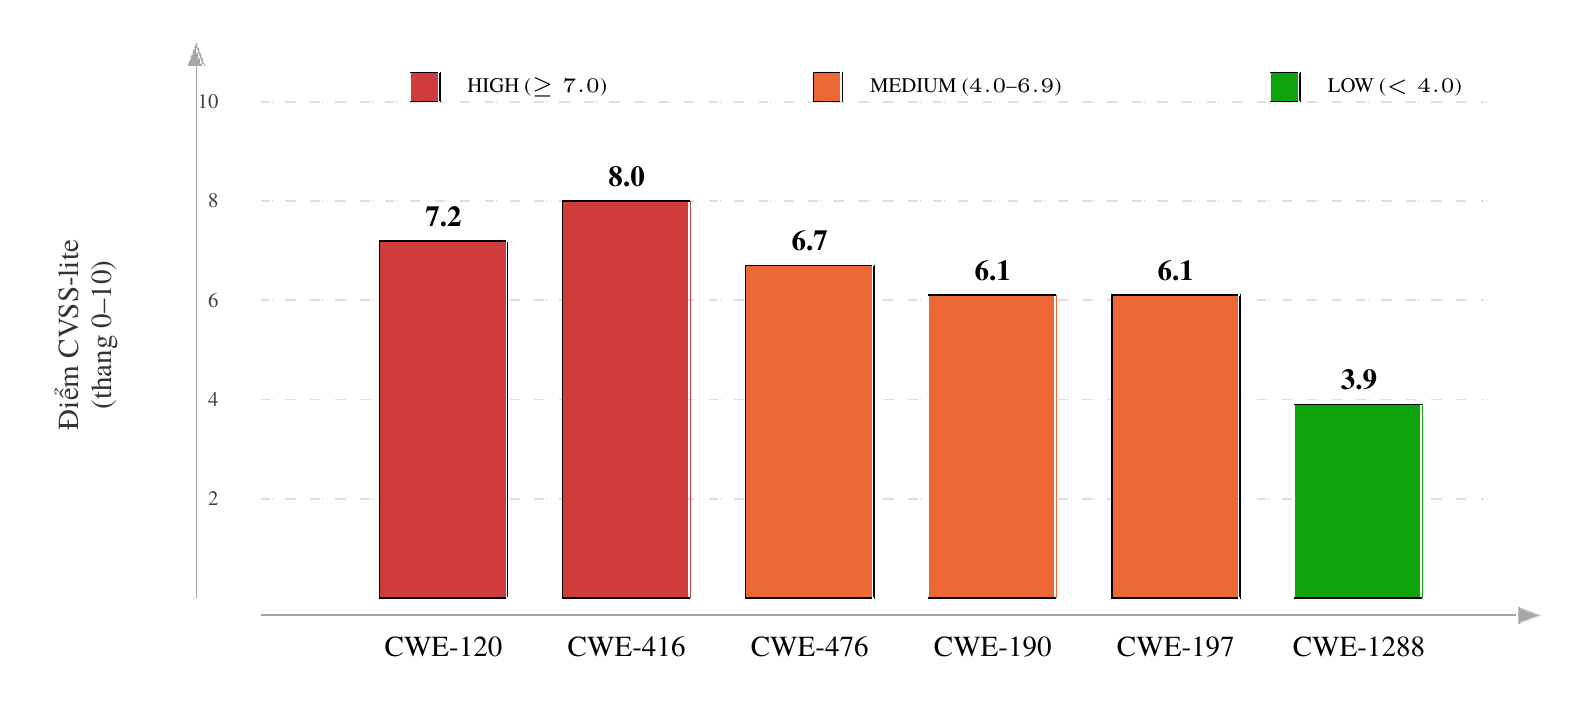
\includegraphics[width=0.85\linewidth]{diagram4_cvss_bar.png}
  \caption{So sánh điểm CVSS-lite giữa 6 CWE của đề tài (số liệu khớp \protect\Cref{tab:cwe-cvss})}
  \label{fig:cvss-bar}
\end{figure}

Nhìn theo biểu đồ: CWE-416 (UAF) và CWE-120 (buffer overflow) là 2 lớp lỗi nghiêm trọng nhất (HIGH, $\geq 7.0$) -- đúng với trực giác vì cả 2 đều có thể dẫn tới hỏng bộ nhớ ngay lập tức; CWE-197 và CWE-190 tuy nguy hiểm nhưng ở mức MEDIUM vì hậu quả quan sát được (sai lệch dữ liệu/DoS) chưa được chứng minh leo thang tới RCE trong phạm vi đề tài (xem hướng mở rộng ở \Cref{sec:thaoluan}).

\begin{table}[H]
  \centering
  \caption{Ví dụ thực tế minh họa cho mỗi lớp CWE}
  \label{tab:cwe-examples}
  \small
  \begin{tabularx}{\linewidth}{@{}l X@{}}
    \toprule
    \textbf{CWE} & \textbf{Ví dụ thực tế minh họa} \\
    \midrule
    CWE-120  & CVE-2003-0352~\cite{cve2003-0352} -- lỗi tràn bộ đệm trong Windows RPC DCOM, bị khai thác bởi worm Blaster \\
    CWE-416  & CVE-2019-0708~\cite{cve2019-0708} (``BlueKeep'') -- use-after-free trong Windows Remote Desktop Services \\
    CWE-476  & Điển hình lớp lỗi DoS phổ biến; xem thêm các ví dụ tại trang CWE-476 của MITRE~\cite{cwe476} \\
    CWE-190  & Ariane 5 Flight 501 (1996)~\cite{ariane5report} -- không phải mã CVE (xảy ra trước khi hệ thống CVE ra đời năm 1999) nhưng là sự cố tràn số nguyên kinh điển nhất từng được ghi nhận \\
    CWE-197  & Chưa xác minh được một CVE công khai khớp chính xác; xem trang CWE-197 của MITRE~\cite{cwe197} \\
    CWE-1288 & Chưa xác minh được một CVE công khai khớp chính xác; xem trang CWE-1288 của MITRE~\cite{cwe1288} \\
    \bottomrule
  \end{tabularx}
\end{table}

\noindent\textit{Lưu ý phương pháp luận:} bảng trên cố ý \textbf{không} gán một mã CVE cụ thể cho CWE-476/197/1288 vì không xác minh được một CVE thực sự khớp chính xác với bối cảnh đề tài trong phạm vi kiểm chứng cho phép -- thà để trống còn hơn trích dẫn một mã CVE không chắc chắn đúng.

\subsection{Ma trận truy vết Test Case $\to$ Yêu cầu (IEEE 829)}
\label{sec:traceability}

Các mục 5.1--5.4 trên trình bày kết quả \emph{theo từng chương/kỹ thuật}. Bảng dưới đây tổ chức lại đúng cùng số liệu đó theo hướng ngược lại -- \emph{theo từng yêu cầu (REQ/NFR)} -- theo tinh thần đặc tả \emph{Test Case Specification} của chuẩn IEEE~829-2008~\cite{ieee829} (mã test case, điều kiện đầu vào, kết quả mong đợi, kết quả thực tế đối chiếu ngược lại nguồn log thật). Đây là góc nhìn truy vết hai chiều REQ $\leftrightarrow$ Test Case còn thiếu ở \Cref{sec:dacta}, nơi mới chỉ đặc tả yêu cầu mà chưa chỉ rõ từng yêu cầu được kiểm chứng bởi test case cụ thể nào.

{\scriptsize
\setlength{\tabcolsep}{3.5pt}
\renewcommand{\arraystretch}{1.35}
\begin{longtable}{@{}
  >{\raggedright\arraybackslash}p{1.3cm}
  >{\raggedright\arraybackslash}p{1.2cm}
  >{\raggedright\arraybackslash}p{3.8cm}
  >{\raggedright\arraybackslash}p{2.3cm}
  >{\raggedright\arraybackslash}p{4.6cm}
  >{\centering\arraybackslash}p{1.1cm}@{}}
  \caption{Ma trận truy vết Test Case $\to$ Yêu cầu (mọi kết quả thực tế trích từ \texttt{logs/*.log} thật)}
  \label{tab:trace} \\
  \toprule
  \textbf{Mã TC} & \textbf{REQ} & \textbf{Input / Điều kiện} & \textbf{Kỳ vọng} & \textbf{Thực tế (nguồn log)} & \textbf{KL} \\
  \midrule
  \endfirsthead
  \multicolumn{6}{l}{\textit{(tiếp theo Bảng~\ref{tab:trace})}} \\
  \toprule
  \textbf{Mã TC} & \textbf{REQ} & \textbf{Input / Điều kiện} & \textbf{Kỳ vọng} & \textbf{Thực tế (nguồn log)} & \textbf{KL} \\
  \midrule
  \endhead
  \midrule
  \multicolumn{6}{r}{\textit{xem tiếp trang sau}} \\
  \endfoot
  \bottomrule
  \endlastfoot
  TC-K1-01 & REQ-1 & BMC $P_1$, bản BUGGY (bước nhảy thẳng sang tính tiền, bỏ qua phân công) & UNSAT (không vi phạm) & \textbf{SAT} -- phản ví dụ $S_0{\to}S_5{\to}S_4$ (\texttt{kripke\_bmc.log}) & FAIL$^*$ \\
  \addlinespace[3pt]
  TC-K1-02 & REQ-1 & BMC $P_1$, bản FIXED & UNSAT & UNSAT (\texttt{kripke\_bmc.log}) & PASS \\
  \addlinespace[3pt]
  TC-K1-03 & REQ-2 & BMC $P_2$, cả 2 bản & UNSAT & UNSAT cả 2 bản (\texttt{kripke\_bmc.log}) & PASS \\
  \addlinespace[3pt]
  TC-K2-01 & REQ-3 & Scanner quét \texttt{strcpy} (\texttt{hoTen}\slash\texttt{maLop}\slash\texttt{bangCap}\slash\texttt{maGiangVien}) trên 3 file VULN & Phát hiện đủ cảnh báo CWE-120 & 5 cảnh báo CWE-120 đúng vị trí (\texttt{pattern\_scanner.log}) & PASS \\
  \addlinespace[3pt]
  TC-K2-02 & REQ-3 & Scanner quét \texttt{main\_fixed.c} & 0 cảnh báo & 0 cảnh báo -- \texttt{[CLEAN]} (\texttt{pattern\_scanner.log}) & PASS \\
  \addlinespace[3pt]
  TC-K4-01 & REQ-3 & White-box Target 1: \texttt{hoTen} dài 81 ký tự $>$ CON-1 (80) & Tìm điều kiện gây tràn & SAT ở lần thử 1 (\texttt{fuzzer\_whitebox.log}) & FAIL$^*$ \\
  \addlinespace[3pt]
  TC-K4-02 & REQ-3 & White-box Target 2: \texttt{maLop} dài 21 ký tự $>$ CON-4 (20) & Tìm điều kiện gây tràn & SAT ở lần thử 2 (\texttt{fuzzer\_whitebox.log}) & FAIL$^*$ \\
  \addlinespace[3pt]
  TC-K4-03 & REQ-3 & Black-box 200 lần ngẫu nhiên trên VULN & 0/200 crash & 72/200 crash, exit \texttt{0xC0000374} (\texttt{fuzzer\_blackbox.log}) & FAIL$^*$ \\
  \addlinespace[3pt]
  TC-K4-04 & REQ-3 & Black-box 200 lần trên FIXED & 0/200 crash & 0/200 crash (\texttt{fuzzer\_blackbox.log}) & PASS \\
  \addlinespace[3pt]
  TC-K2-03 & REQ-4 & Scanner quét \texttt{dangling\_free} trên VULN & Phát hiện CWE-416 tại \texttt{giang\_vien.c:35} & Phát hiện đúng vị trí (\texttt{pattern\_scanner.log}) & PASS \\
  \addlinespace[3pt]
  TC-K4-05 & REQ-4 & White-box Target 3: \texttt{free(gv)} rồi vẫn đọc qua \texttt{gv\_ptr} & Tìm điều kiện UAF & SAT ở lần thử 3 (\texttt{fuzzer\_whitebox.log}) & FAIL$^*$ \\
  \addlinespace[3pt]
  TC-K2-04 & REQ-4 & \texttt{memory\_trace\_demo.py}: đọc \texttt{gv->hoTen} sau \texttt{free()}, bản ASan-VULN & ASan phải bắt lỗi & \texttt{heap-use-after-free}, ABORTING, offset $+24$ byte $=$ \texttt{hoTen} (\texttt{memory\_trace.log}) & FAIL$^*$ \\
  \addlinespace[3pt]
  TC-K2-05 & REQ-4 & \texttt{memory\_trace\_demo.py}, bản ASan-FIXED (\texttt{gv\_ptr=NULL} trước free) & 0 vi phạm & 0 vi phạm (\texttt{memory\_trace.log}) & PASS \\
  \addlinespace[3pt]
  TC-K2-06 & REQ-5 & Scanner quét \texttt{unchecked\_\allowbreak nested\_\allowbreak deref} trên VULN & Phát hiện CWE-476 tại \texttt{tinh\_tien\_day.c:13} & Phát hiện đúng vị trí (\texttt{pattern\_scanner.log}) & PASS \\
  \addlinespace[3pt]
  TC-K4-06 & REQ-5 & White-box Target 4: \texttt{gv\_ptr=NULL} rồi gọi \texttt{calculate\_e2e\_salary} & Tìm điều kiện NULL deref & SAT ở lần thử 4 (\texttt{fuzzer\_whitebox.log}) & FAIL$^*$ \\
  \addlinespace[3pt]
  TC-K3-01 & REQ-6 & Check 1 (Z3): $\exists$ input hợp lệ làm tràn \texttt{int32} & SAT dự kiến (đang kiểm định code VULN) & SAT -- numClasses=20, soTiet=120 (\texttt{smt\_verify.log}) & FAIL$^*$ \\
  \addlinespace[3pt]
  TC-K3-02 & REQ-6 & Check 2 (Z3): cùng câu hỏi trên \texttt{long long} (bản vá) & UNSAT & UNSAT (\texttt{smt\_verify.log}) & PASS \\
  \addlinespace[3pt]
  TC-K4-07 & REQ-6 & White-box Target 5: soTiet=16694179, dmt=2147583020 & SAT dự kiến & SAT ở lần thử 5 (\texttt{fuzzer\_whitebox.log}) & FAIL$^*$ \\
  \addlinespace[3pt]
  TC-K1-04 & REQ-8 & BMC $P_5$, bản VULN & UNSAT & SAT -- $S_3$ mang nhãn \texttt{byte\_truncated} (\texttt{kripke\_bmc.log}) & FAIL$^*$ \\
  \addlinespace[3pt]
  TC-K1-05 & REQ-8 & BMC $P_5$, bản FIXED & UNSAT & UNSAT (\texttt{kripke\_bmc.log}) & PASS \\
  \addlinespace[3pt]
  TC-K3-03 & REQ-8 & Check 4 (Z3): $\exists\, n\in[0,300]$ ép kiểu \texttt{char} sai giá trị & SAT dự kiến & SAT -- $n=128 \to$ byte $=-128$ (\texttt{smt\_verify.log}) & FAIL$^*$ \\
  \addlinespace[3pt]
  TC-K3-04 & REQ-8 & Check 5 (Z3): cùng câu hỏi với guard $[0,127]$ & UNSAT & UNSAT (\texttt{smt\_verify.log}) & PASS \\
  \addlinespace[3pt]
  TC-K3-05 & REQ-8, NFR-5 & Check 6 (Z3): $\exists\, a\ne b \in [0,300]$ cùng cho 1 byte & UNSAT mong muốn (an toàn truy vết) & SAT -- $a=0, b=256$ cùng byte $=0$ (\texttt{smt\_verify.log}) & FAIL$^{**}$ \\
  \addlinespace[3pt]
  TC-K4-08 & REQ-8 & Black-box CWE-197, 200 lần trên VULN & 0/200 sai lệch & 120/200 sai lệch, 60\% (\texttt{fuzzer\_blackbox.log}) & FAIL$^*$ \\
  \addlinespace[3pt]
  TC-K4-09 & REQ-8 & Black-box CWE-197, 200 lần trên FIXED & 0/200 sai lệch & 0/200 sai lệch, 146/200 chặn an toàn (\texttt{fuzzer\_blackbox.log}) & PASS \\
  \addlinespace[3pt]
  TC-K4-10 & REQ-8, NFR-5 & BVA 17 giá trị biên cố định trên VULN & Byte thật khớp byte tính tay 17/17; không nên trùng lặp & 17/17 khớp lý thuyết, nhưng lộ 6 nhóm trùng lặp byte thật (\texttt{fuzzer\_blackbox.log}) & PASS\slash FAIL$^{**}$ \\
  \addlinespace[3pt]
  TC-K4-11 & REQ-8, NFR-5 & BVA 17 giá trị biên trên FIXED & 0 nhóm trùng lặp & 0 nhóm trùng lặp (\texttt{fuzzer\_blackbox.log}) & PASS \\
  \addlinespace[3pt]
  TC-K3-06 & REQ-9 & Check 7 (Z3): $\exists$ 2 danh mục \texttt{bangCap} khác nhau (\texttt{CU\_NHAN} thật, chuỗi không hợp lệ) cùng cho 1 \texttt{heSoBangCap} & UNSAT mong muốn (phân biệt được) & SAT -- cả 2 cùng rơi vào fallback $1.0$ (\texttt{smt\_verify.log}) & FAIL$^{**}$ \\
  \addlinespace[3pt]
  TC-K4-12 & REQ-9 & Black-box: \texttt{bangCap} ngẫu nhiên gồm giá trị không hợp lệ, trên VULN & Cần oracle xác nhận hệ thống xử lý đúng & Script chỉ đếm 74/200 lần input không hợp lệ được sinh ra (không crash), KHÔNG assert hành vi đúng/sai (\texttt{fuzzer\_blackbox.log}) & QS$^\dagger$ \\
  \addlinespace[3pt]
  TC-K2-07 & REQ-7 & (chưa có test case riêng) & Công thức tính lương đúng với mọi input hợp lệ & Check 1/2 chỉ chứng minh KHÔNG TRÀN SỐ, không chứng minh giá trị tính ra khớp công thức nghiệp vụ mong đợi & QS$^\dagger$ \\
  \addlinespace[3pt]
  TC-N01 & NFR-1 & \texttt{e2e\_nfr\_bench 10000} trên \texttt{salary\_calc\_fixed.exe} (\texttt{QueryPerformanceCounter}) & Trung bình $<10\,$ms/lần & $0{,}000014\,$ms/lần (\texttt{nfr\_check.log}) & PASS \\
  \addlinespace[3pt]
  TC-N02 & NFR-1 & \texttt{e2e\_nfr\_bench 10000} trên \texttt{salary\_calc.exe} (VULN, đối chứng) & Trung bình $<10\,$ms/lần & $0{,}000011\,$ms/lần (\texttt{nfr\_check.log}) & PASS \\
  \addlinespace[3pt]
  TC-N03 & NFR-2 & $10\,000$ lần tạo/xoá \texttt{GiangVien}+\texttt{LopHocPhan} trên bản FIXED, đo \texttt{GetProcessMemoryInfo} & Drift $<1024$\,KB & Drift $=4$\,KB (\texttt{nfr\_check.log}) & PASS \\
  \addlinespace[3pt]
  TC-N04 & NFR-2 & Cùng kịch bản trên bản VULN (đối chứng -- CWE-416 là dangling pointer, không phải leak) & Drift $<1024$\,KB & Drift $=4$\,KB (\texttt{nfr\_check.log}) & PASS \\
\end{longtable}
}

\noindent\footnotesize $^*$FAIL trên bản BUGGY/VULN là kết quả \emph{đúng như thiết kế}: đây là bug injection có chủ đích để minh chứng công cụ phát hiện được lỗi thật, không phải lỗi của bản thân test case hay công cụ kiểm chứng. $^{**}$FAIL phản ánh một giới hạn thiết kế thật (chỉ dùng 1 byte để lưu audit log, xem NFR-5 và \Cref{sec:thaoluan}), không phải lỗi hiện thực có thể vá bằng guard đơn giản như CWE-197 gốc. $^\dagger$QS = Quan sát: đề tài hiện \textbf{chưa có oracle tự động} assert Pass/Fail cho REQ-7 (đúng công thức tính lương) và REQ-9 (validate \texttt{bangCap}) -- đây là hai khoảng hở truy vết thật, được phát hiện chính nhờ việc lập ma trận này theo chiều REQ $\to$ Test Case, không phải hai yêu cầu này chưa từng được đề cập ở nơi khác trong báo cáo.\normalsize

\section{Thảo luận và Hạn chế}
\label{sec:thaoluan}

\subsection{Giới hạn phương pháp}

\begin{itemize}
  \item \textbf{BMC $k=5$ chưa đạt completeness threshold}: kết quả \textbf{UNSAT} của BMC chỉ chứng minh ``không có vi phạm trong $k=5$ bước'', \emph{không} loại trừ khả năng tồn tại vi phạm ở bước sâu hơn -- đây chính là lý do $P_3$ (Liveness) ra SAT ở cả 2 bản (\Cref{sec:ketqua}): BMC hữu hạn không thể chứng minh một thuộc tính ``cuối cùng phải xảy ra'' một cách tuyệt đối, chỉ có thể chứng minh trong phạm vi $k$ bước đã duyệt.
  \item \textbf{Pattern scanner dùng regex/so khớp chuỗi, không phải phân tích AST/data-flow liên hàm (interprocedural) đầy đủ}: công cụ chỉ xét được guard-check trong phạm vi \emph{một hàm}, nên sẽ bỏ sót lớp lỗi mà điều kiện bảo vệ nằm ở một hàm gọi \emph{khác} với hàm chứa điểm truy cập nguy hiểm (ví dụ: một hàm kiểm tra \texttt{gv\_ptr != NULL} rồi truyền tiếp con trỏ đã kiểm tra sang một hàm thứ hai đọc nó -- scanner hiện tại sẽ không ``nhớ'' guard đó qua ranh giới lời gọi hàm). Đây là giới hạn cấu trúc cố hữu của một scanner một-pass; công cụ phù hợp để bổ trợ chứ không thay thế một static analyzer thật (Clang Static Analyzer, cppcheck với chế độ \texttt{--enable=all}).
  \item \textbf{Fuzzing trên Windows dùng exit code thay vì tín hiệu SIGSEGV kiểu POSIX}: Windows không có SIGSEGV theo nghĩa POSIX cho crash native; toàn bộ 72 mẫu crash CWE-120 quan sát được ở Chương 4 đều trả về \textbf{cùng một exit code 3221226356} (\texttt{0xC0000374} -- \texttt{STATUS\_HEAP\_CORRUPTION}), không phải \texttt{0xC0000005} (\texttt{STATUS\_ACCESS\_VIOLATION}) như trực giác thường nghĩ về ``buffer overflow gây segfault''. Điều này phản ánh đúng cơ chế Windows CRT heap: ghi tràn qua \texttt{hoTen[80]} làm hỏng heap metadata liền kề, và lỗi chỉ bị phát hiện \emph{muộn hơn} -- tại lần gọi \texttt{free()} kế tiếp khi CRT heap manager kiểm tra tính toàn vẹn metadata -- chứ không crash ngay tại dòng \texttt{strcpy}. Đây cũng là lý do một phần các lần thử ``overflow'' không crash ngay (75/200 rơi vào nhánh ``logic error'' thay vì crash): tuỳ lượng dữ liệu ghi tràn có chạm đúng vùng metadata bị kiểm tra hay không.
\end{itemize}

\subsection{So sánh với lý thuyết đã học}

\begin{itemize}
  \item Kết quả $P_3$ SAT ở cả 2 bản đúng với lý thuyết \emph{Soundness/Completeness} của BMC đã học ở Chương 1: BMC là \emph{sound nhưng không complete} đối với Liveness ở độ sâu hữu hạn -- một kết quả SAT ở $P_3$ không tự động suy ra lỗi mã nguồn, phải phân biệt rõ với SAT của các thuộc tính Safety ($P_1,P_2,P_4,P_5$) vốn luôn tương ứng phản ví dụ thật.
  \item Tốc độ tăng tốc $\approx 30.5\times$ của white-box so với black-box phù hợp đúng dự đoán lý thuyết Chương 4: constraint solving trực tiếp (giải 7 ràng buộc đã biết) về bản chất là $O(1)$ theo số lần gọi solver, trong khi random fuzzing là $O(n)$ theo số lần thử cần để ngẫu nhiên trúng đúng điều kiện biên -- tỉ lệ tăng tốc dao động khá lớn giữa các lần chạy thực tế (quan sát được từ $\approx 30\times$ đến $\approx 280\times$ tuỳ độ trễ khởi tạo tiến trình con của Windows ở từng lần đo) nhưng bản chất định tính không đổi.
\end{itemize}

\subsection{Hướng cải thiện}

\begin{itemize}
  \item Áp dụng \textbf{$k$-Induction} (hoặc chuyển đổi sang Büchi automata) để chứng minh $P_3$ (Liveness) một cách tuyệt đối thay vì chỉ trong phạm vi $k=5$ bước.
  \item Chạy lại bộ fuzzing trên \textbf{Linux} (qua WSL hoặc máy ảo) để thu được tín hiệu \texttt{SIGSEGV}/\texttt{SIGABRT} chuẩn POSIX, đối chiếu trực tiếp với hành vi \texttt{STATUS\_HEAP\_CORRUPTION} đã quan sát trên Windows -- làm rõ liệu sự khác biệt về cơ chế phát hiện lỗi giữa 2 hệ điều hành có ảnh hưởng tới tỉ lệ crash đo được hay không.
  \item Thay thế/bổ trợ \texttt{pattern\_scanner.py} bằng một static analyzer thật hỗ trợ phân tích interprocedural (cppcheck~\cite{cppcheck} \texttt{--enable=all} hoặc Clang Static Analyzer) để mở rộng phạm vi phát hiện ra ngoài giới hạn ``một hàm'' đã nêu ở mục 6.1.
  \item Mở rộng bảng CVSS-lite (\Cref{tab:cwe-cvss}) bằng việc thực sự khai thác (exploit) thử một lỗ hổng CWE-120 thành RCE có kiểm soát trong môi trường cô lập, để có cơ sở thực nghiệm nâng điểm Impact (C/I) thay vì chỉ dựa trên crash/DoS đã quan sát.
\end{itemize}

\section{Kết luận}
\label{sec:ketluan}

Đề tài đã phân tích và kiểm chứng an toàn mô-đun tính thù lao giảng viên của hệ thống DuongUniversity Management System bằng 4 kỹ thuật kiểm chứng bổ sung cho nhau -- mô hình hóa hình thức (Kripke/BMC), phân tích tĩnh (pattern scanner), kiểm chứng hình thức bằng SMT (Z3), và kiểm thử động (fuzzing black-box/white-box) -- áp dụng đồng nhất trên cùng một hệ thống E2E 3 module thay vì các ví dụ minh họa rời rạc.

Kết quả đạt được: phát hiện và khắc phục thành công \textbf{6 lớp lỗ hổng} (\textbf{CWE-120, CWE-416, CWE-476, CWE-190, CWE-1288, CWE-197}), xác nhận bằng \textbf{9/9 cảnh báo tĩnh} đúng vị trí trên code VULN và \textbf{0 cảnh báo} trên \texttt{main\_fixed.c}; \textbf{5/5 thuộc tính BMC an toàn} trên bản FIXED (chỉ $P_3$ Liveness còn giới hạn kỹ thuật đã giải thích ở \Cref{sec:thaoluan}); \textbf{7 phép chứng minh Z3} xác nhận hình thức cả tồn tại lỗi (Check 1, 4, 6, 7 SAT) lẫn loại trừ hoàn toàn lỗi sau vá (Check 2, 3, 5 UNSAT); và bằng chứng thực nghiệm động qua fuzzing (72/200 crash trên bản lỗi, 0/200 trên bản vá) cùng chẩn đoán thật từ AddressSanitizer (\texttt{heap-use-after-free} được công cụ độc lập xác nhận, không phải tự báo cáo).

Điểm mấu chốt về phương pháp luận: \textbf{4 tầng kiểm chứng cùng đi đến một kết luận nhất quán} -- Chương 1 chứng minh vi phạm ở mức logic điều khiển, Chương 2 chỉ đúng vị trí trên mã nguồn, Chương 3 chứng minh toán học trên toàn miền giá trị, Chương 4 xác nhận biểu hiện thật trên binary đã biên dịch. Không một kỹ thuật nào trong 4 kỹ thuật trên đủ để tự mình bao phủ toàn bộ không gian lỗi có thể có (mỗi kỹ thuật có giới hạn riêng, đã nêu ở \Cref{sec:thaoluan}); sự kết hợp của cả 4 mới tạo thành một quy trình kiểm chứng an toàn phần mềm đáng tin cậy.


\bibliographystyle{plain}
\bibliography{refs/references}
\nocite{*}

\end{document}
